\newpage
%\setlength{\textwidth}{22cm}
\newgeometry{left=1cm, right = 1cm, top = 1cm, bottom = 2cm}

\section{Appendix}

\subsection{A: SEM Images Fabrication Results}
\subsubsection*{A1: PdNb}

\begin{figure}[h]
     \centering
     \begin{subfigure}[b]{\textwidth}
         \centering
         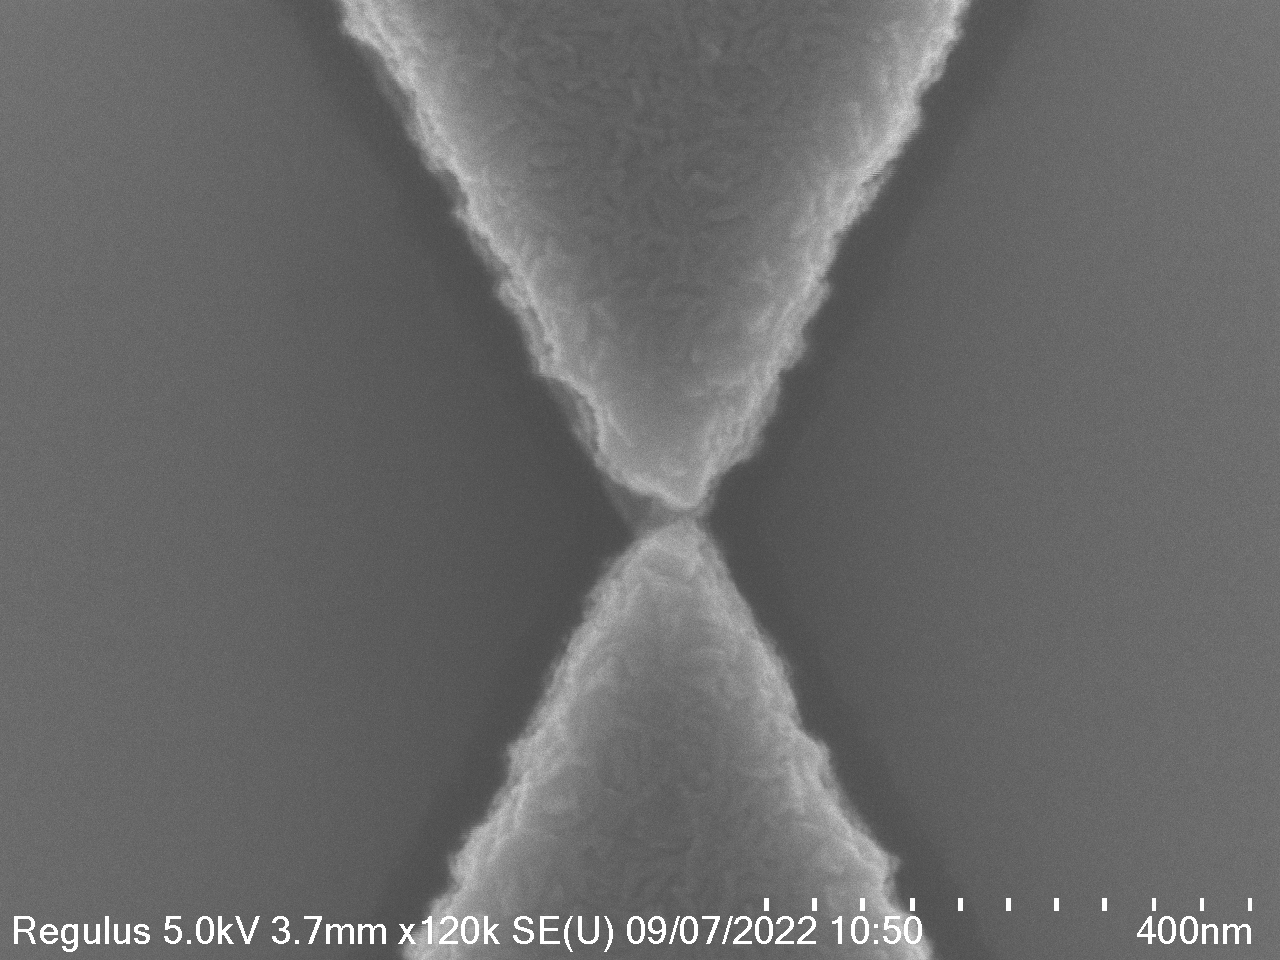
\includegraphics[width=0.32\textwidth]{TiPdPdNbSEMBJ1_31_1300uCcm2_0003_1.png}
         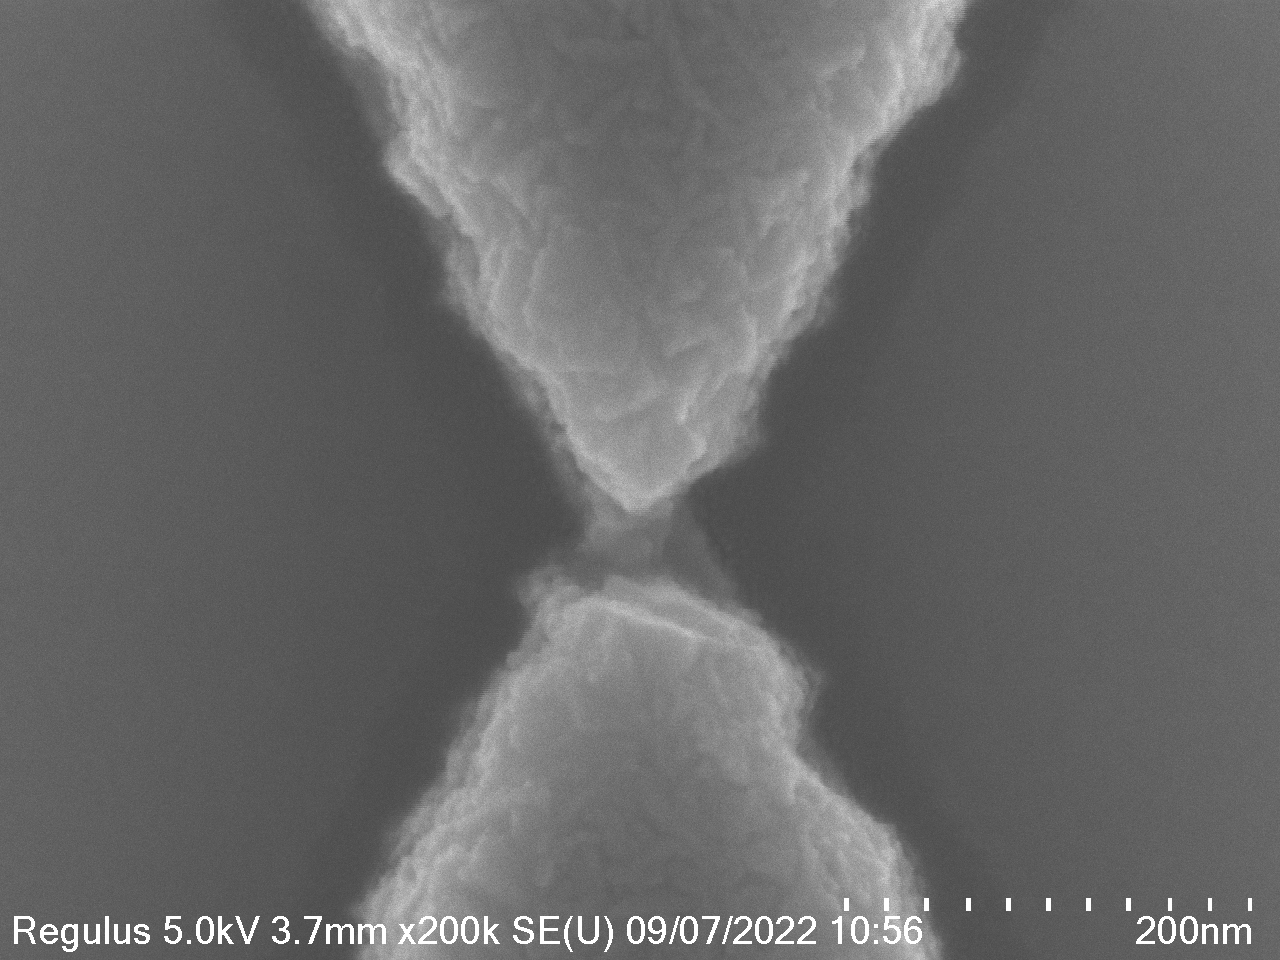
\includegraphics[width=0.32\textwidth]{TiPdPdNbSEMBJ1_31_1320uCcm2_0001_1.png}
         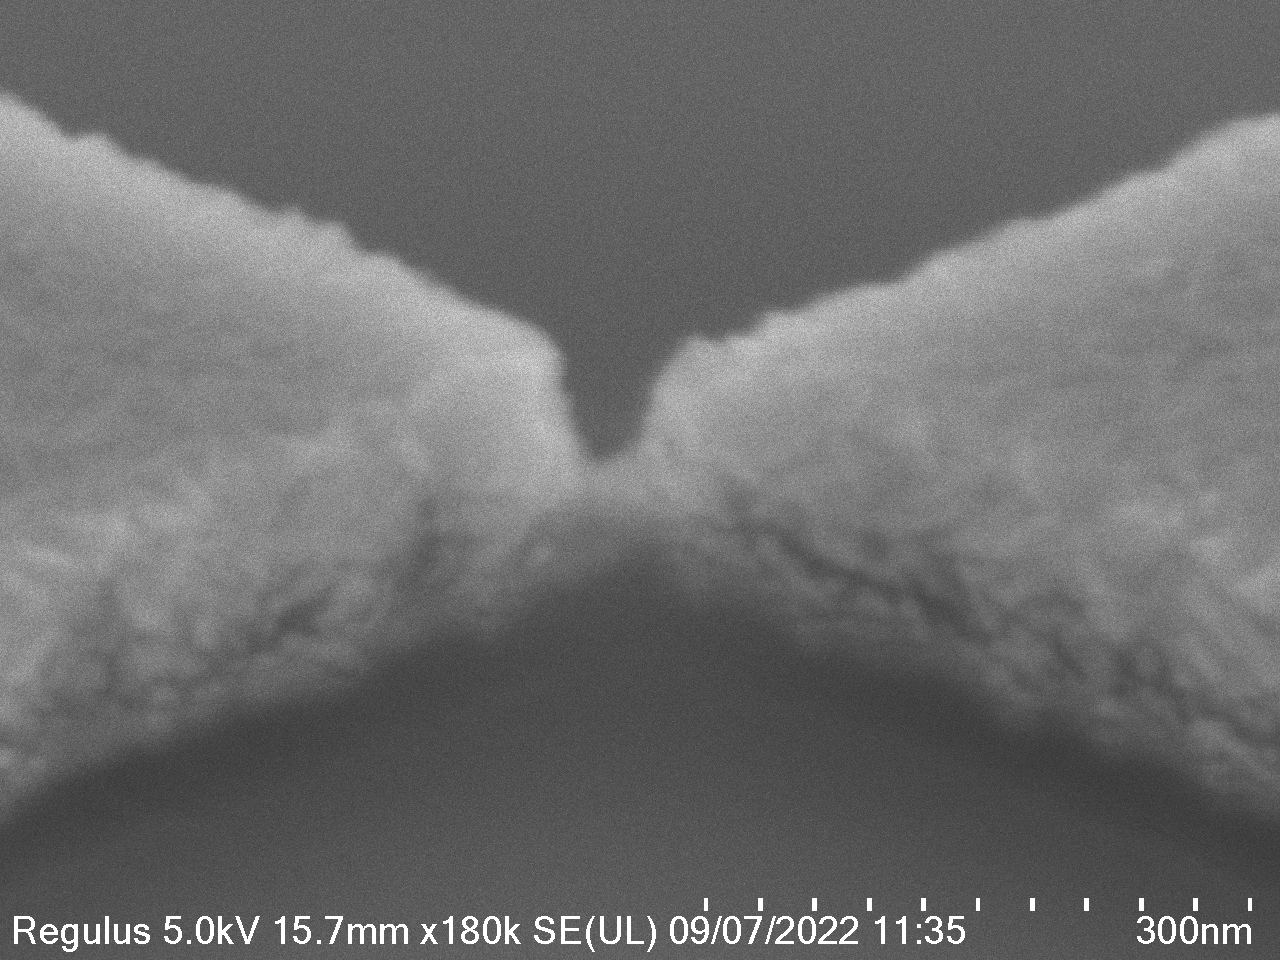
\includegraphics[width=0.32\textwidth]{TiPdPdNbSEMBJ1_31_1320uCcm2_0013_1.png}
         %\caption{A portion of the resist is irradiated with an electron beam in as specified pattern.}
         %\label{c}
     \end{subfigure}
     %\hfill
     \begin{subfigure}[b]{\textwidth}
         \centering
         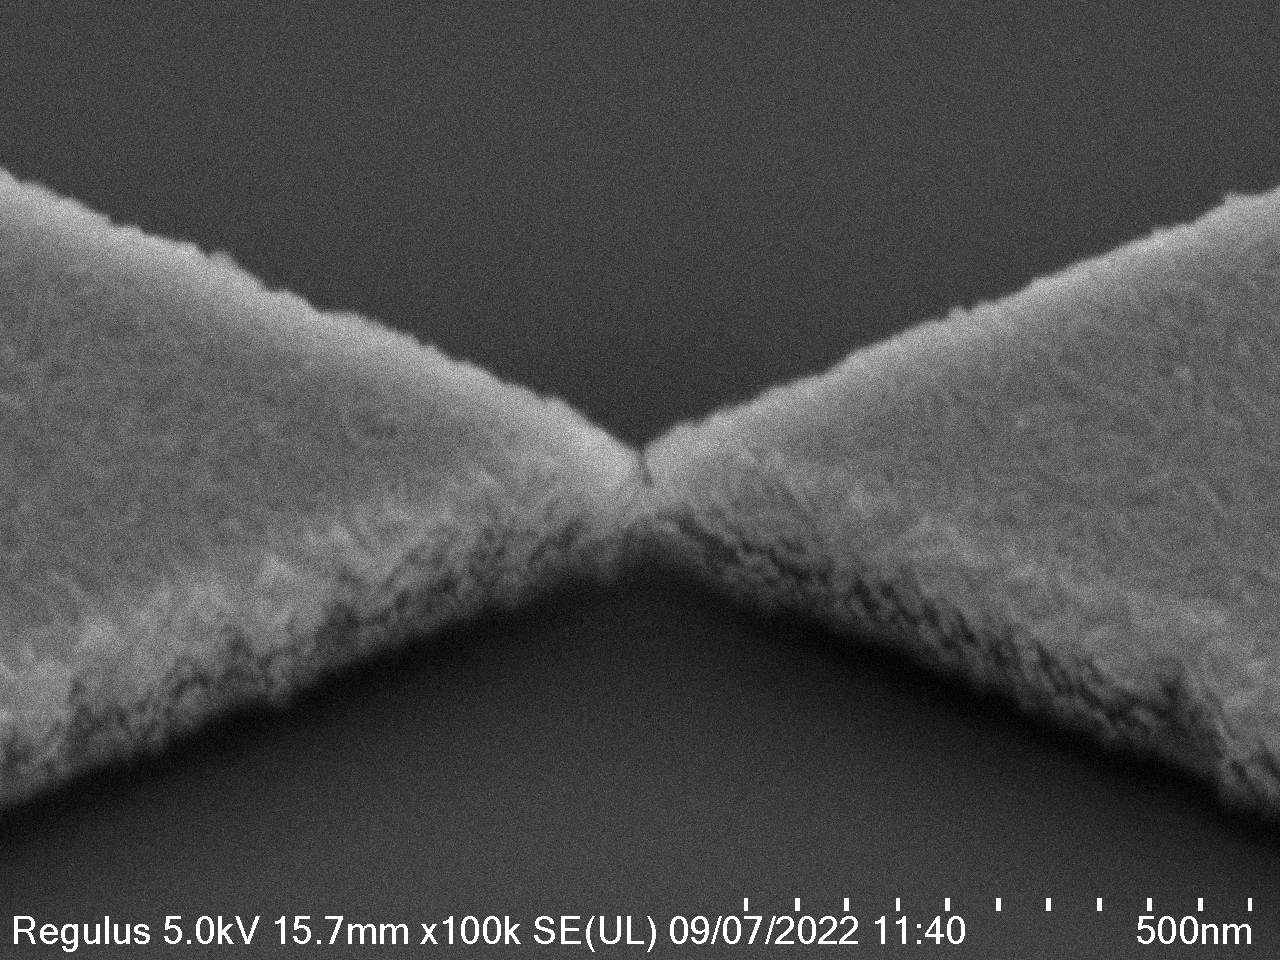
\includegraphics[width=0.32\textwidth]{TiPdPdNbSEMBJ1_31_1340uCcm2_0002_1.png}
         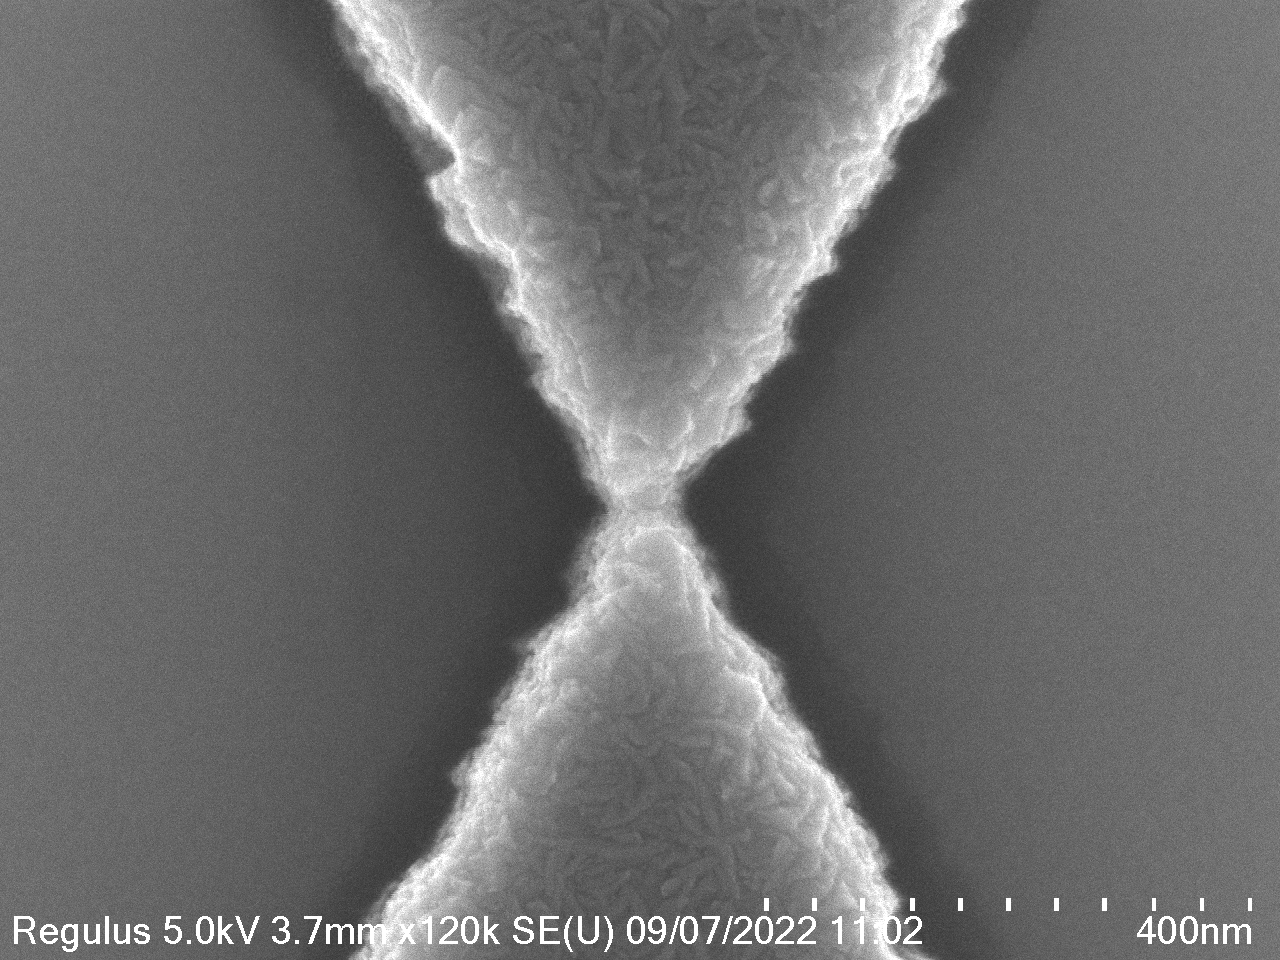
\includegraphics[width=0.32\textwidth]{TiPdPdNbSEMBJ1_31_1660uCcm2_0002_1.png}
         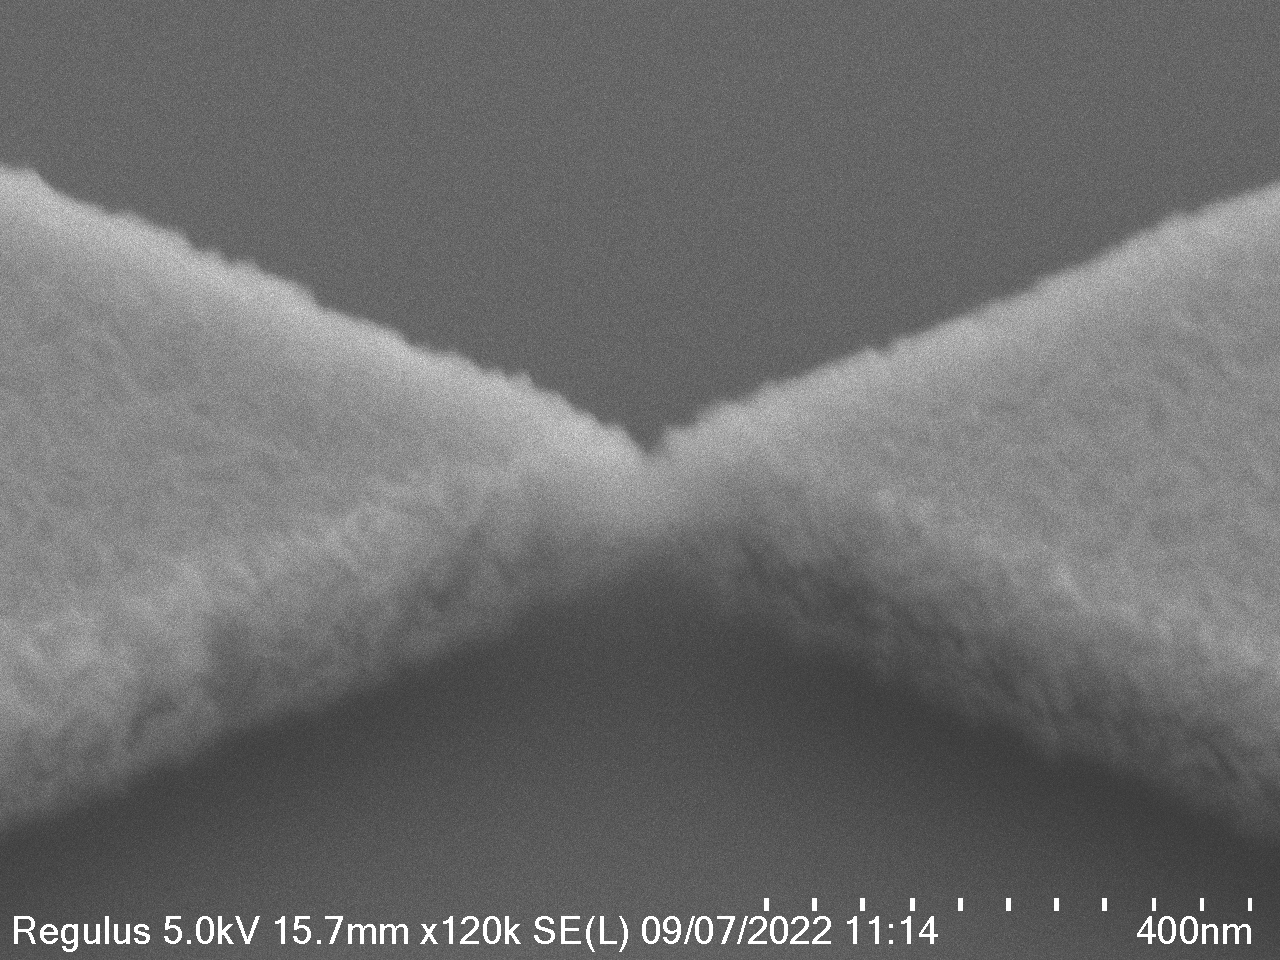
\includegraphics[width=0.32\textwidth]{TiPdPdNbSEMBJ1_31_1660uCcm2_0006_1.png}
         %\caption{A portion of the resist is irradiated with an electron beam in as specified pattern.}
         %\label{c}
     \end{subfigure}
        \caption{SEM images of PdNb devices.}
        \label{fig:}
        
\end{figure}
\vspace{-1cm}

\subsubsection*{A2: AuNb, 100 nm Nb}

\begin{figure}[H]
     \centering
     \begin{subfigure}[b]{\textwidth}
         \centering
         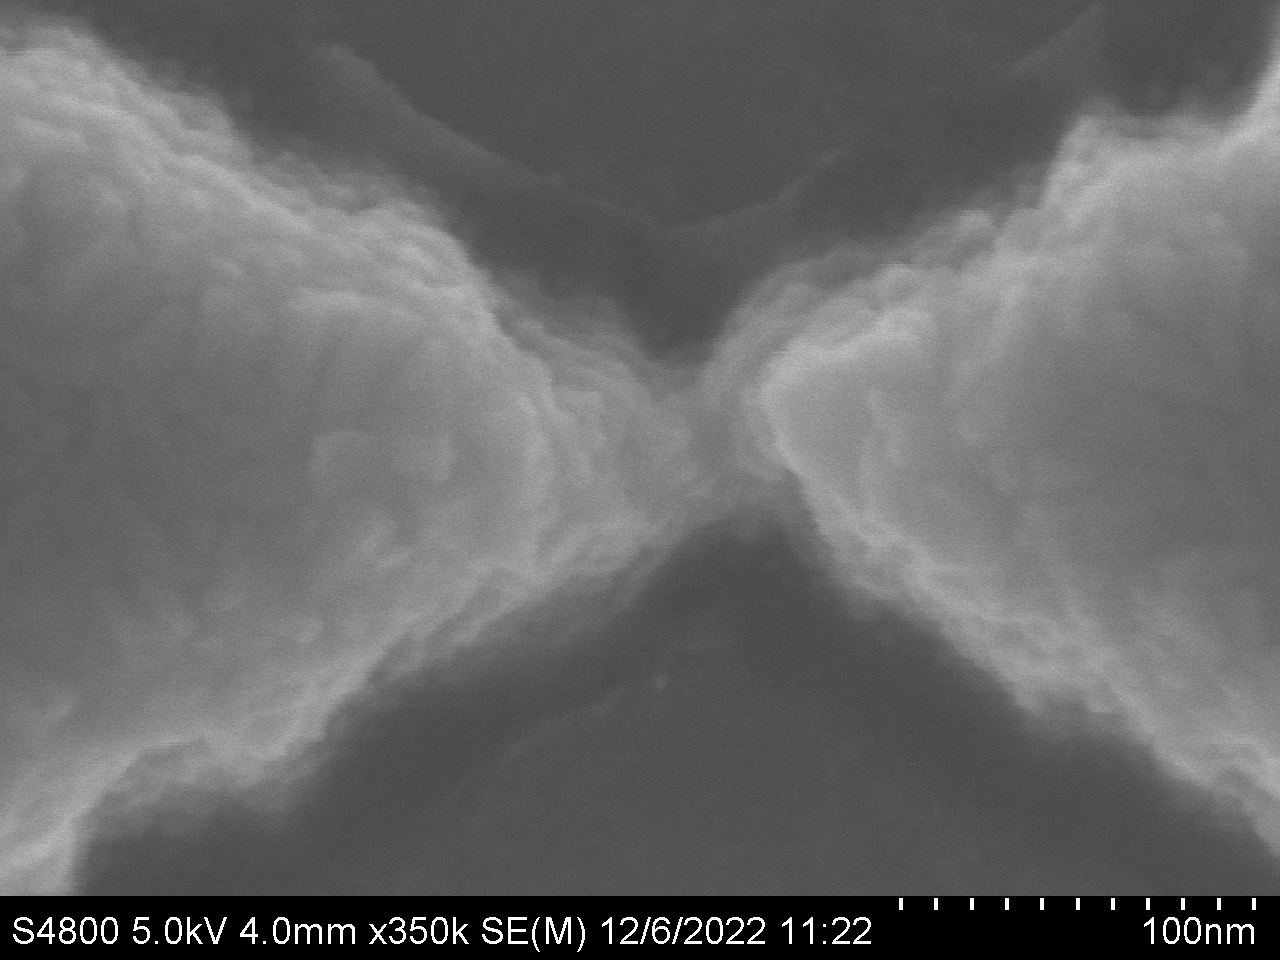
\includegraphics[width=0.32\textwidth]{Appendix_A/A2.png}
         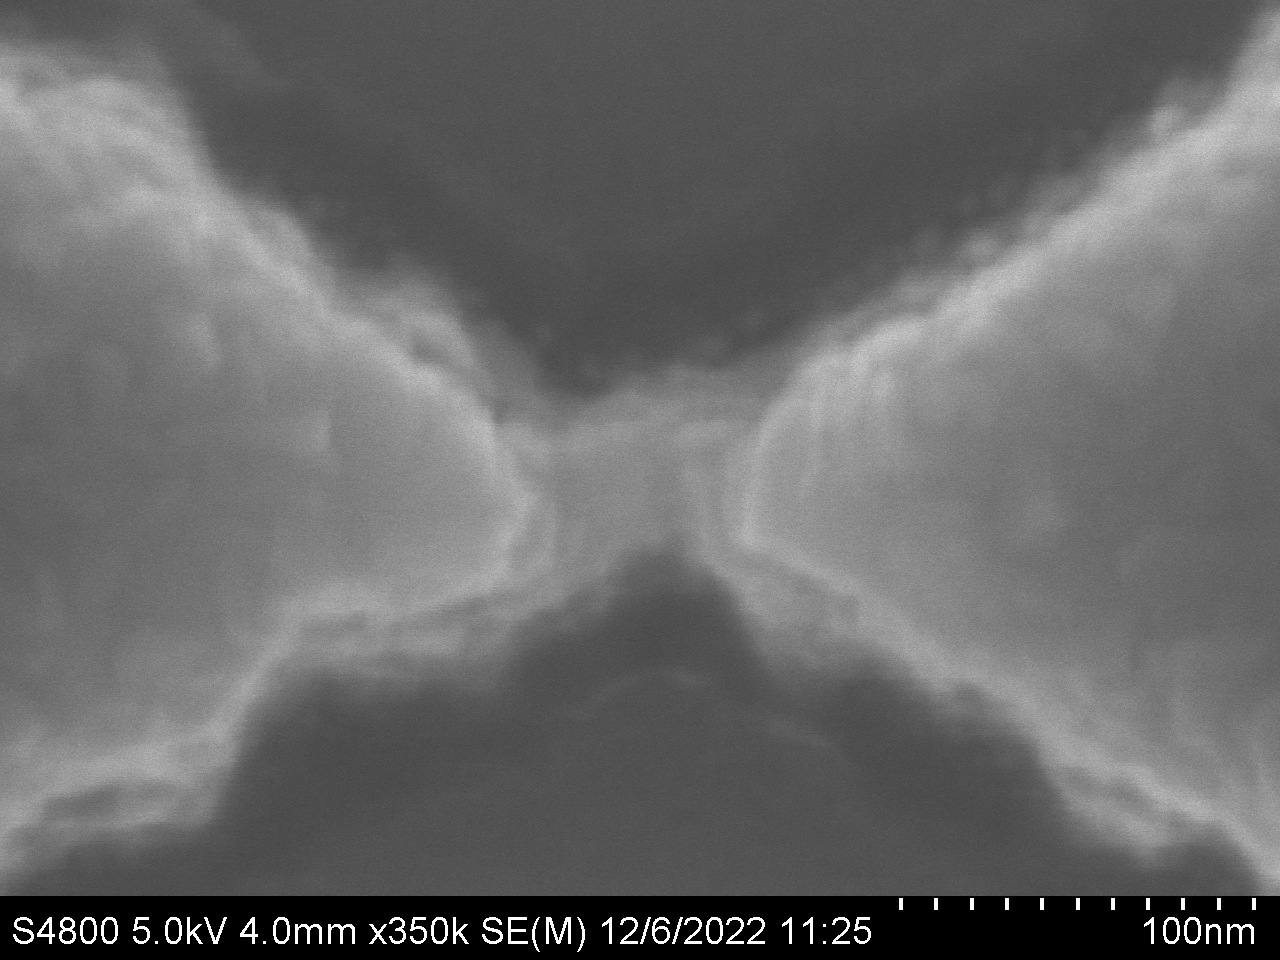
\includegraphics[width=0.32\textwidth]{Appendix_A/A5.png}
         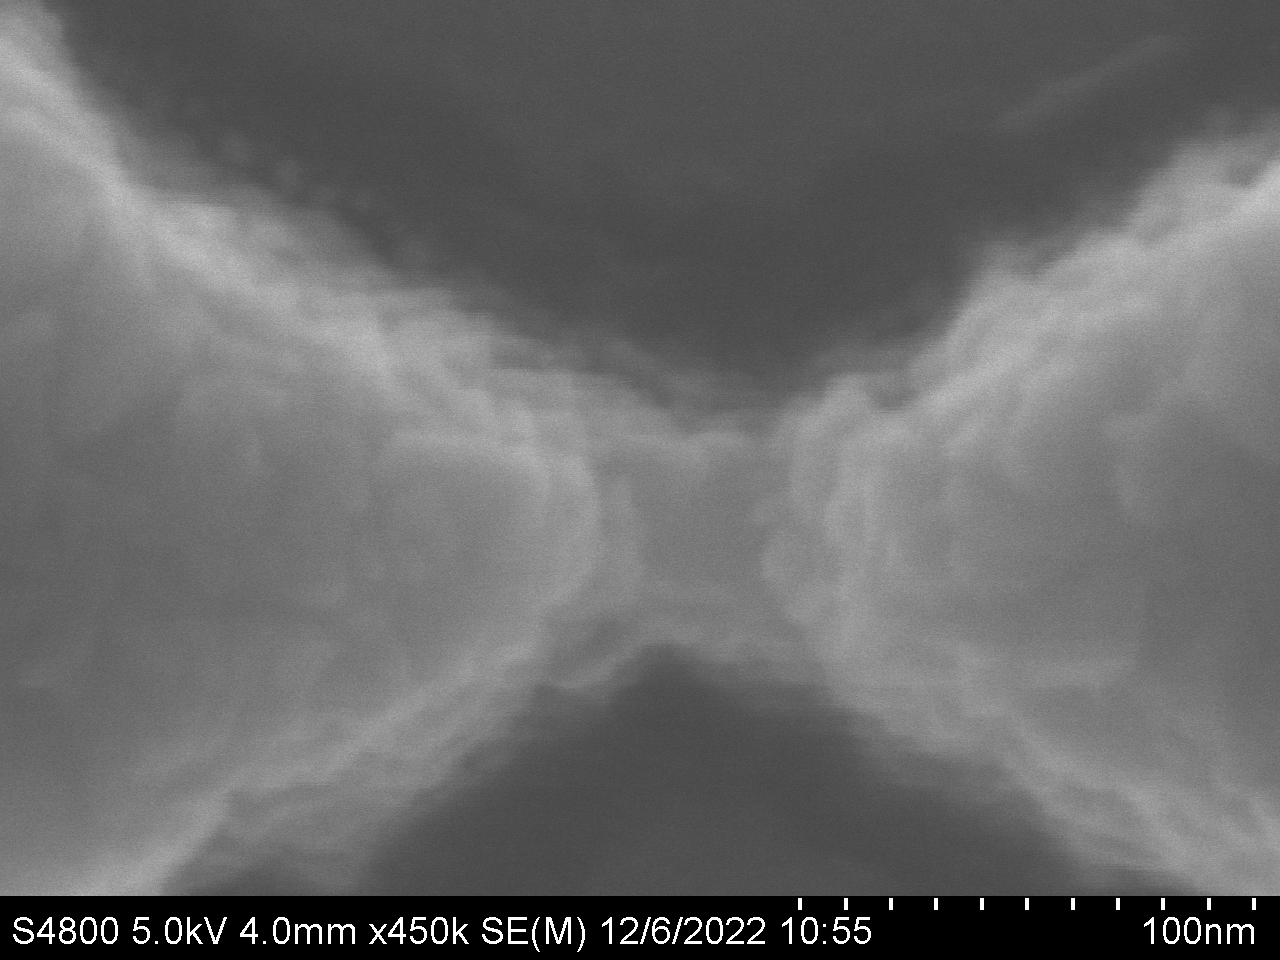
\includegraphics[width=0.32\textwidth]{Appendix_A/E4.png}
         %\caption{A portion of the resist is irradiated with an electron beam in as specified pattern.}
         %\label{c}
     \end{subfigure}
     %\hfill
     \begin{subfigure}[b]{\textwidth}
         \centering
         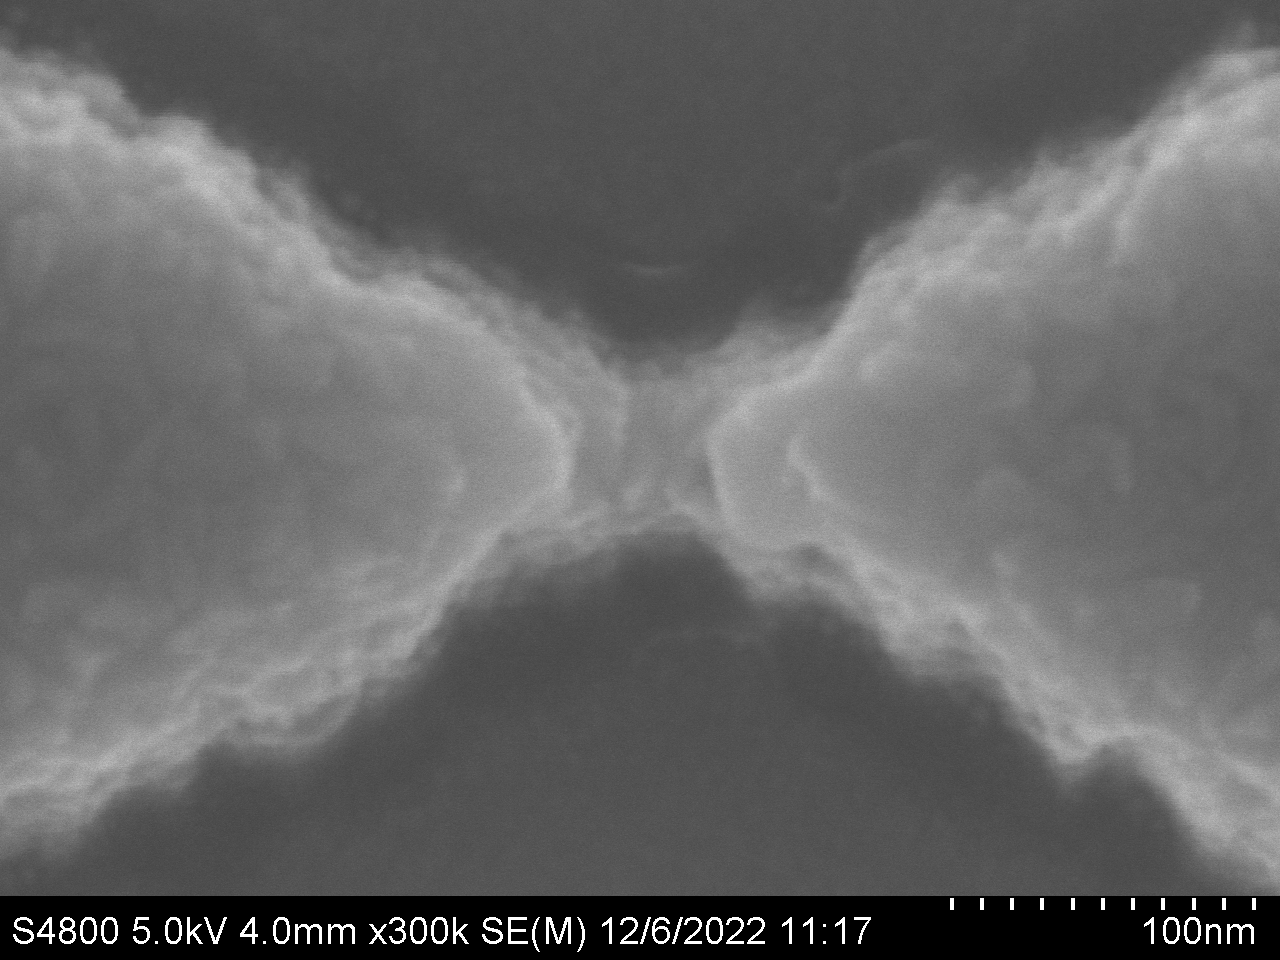
\includegraphics[width=0.32\textwidth]{Appendix_A/C1.png}
         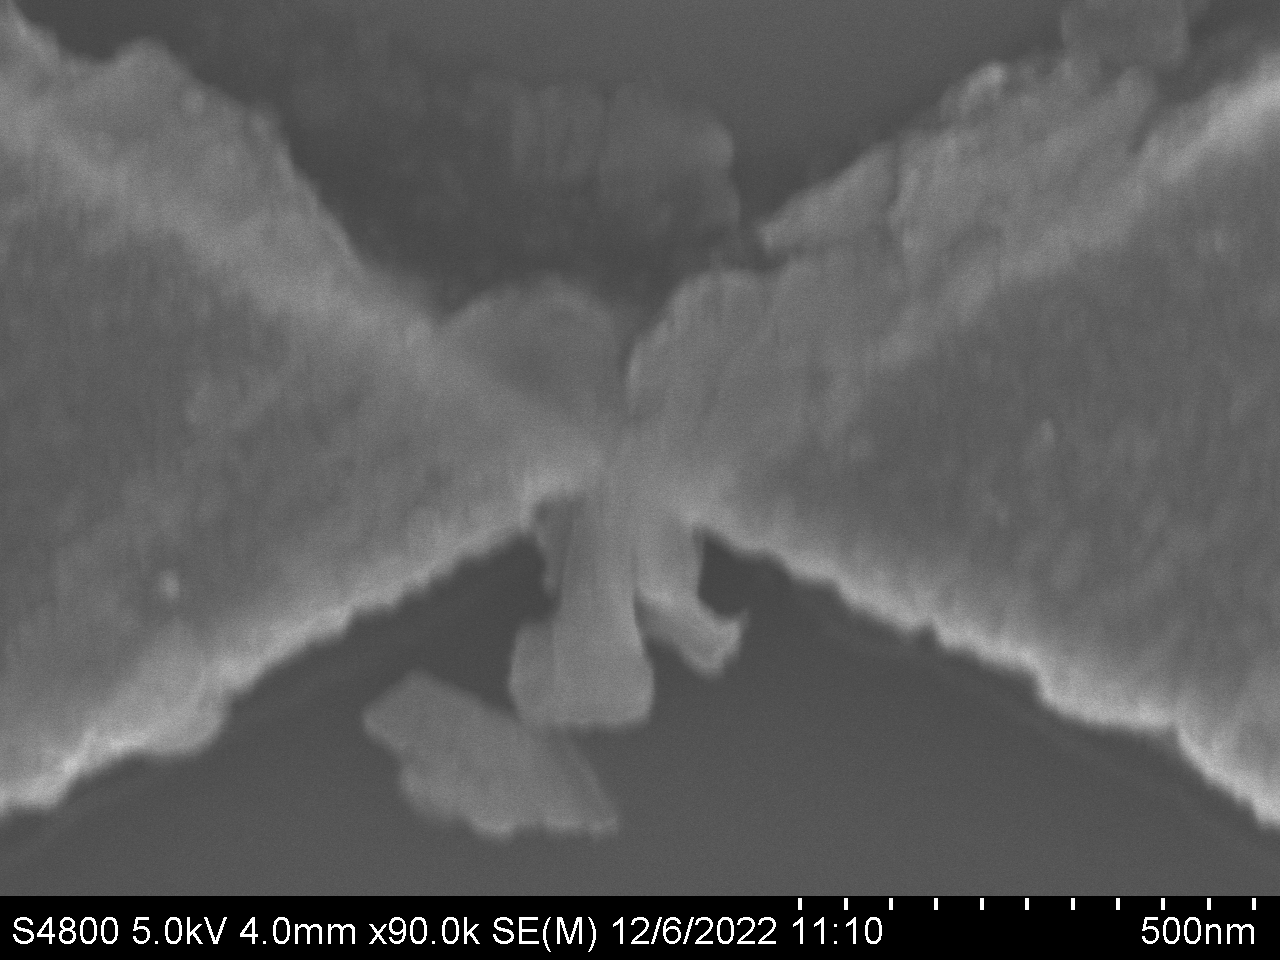
\includegraphics[width=0.32\textwidth]{Appendix_A/D8_2.png}
         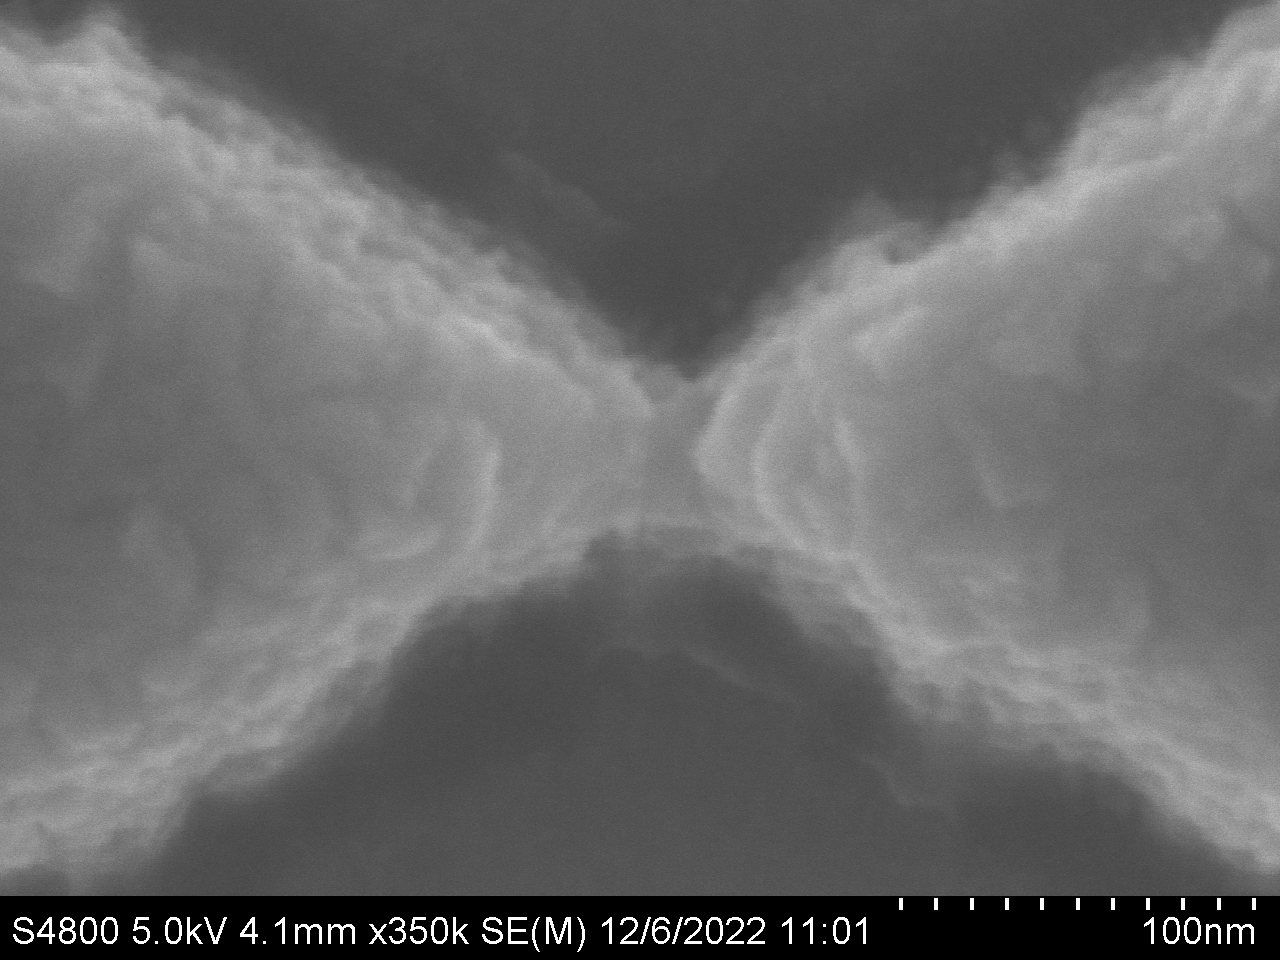
\includegraphics[width=0.32\textwidth]{Appendix_A/E6.png}
         %\caption{A portion of the resist is irradiated with an electron beam in as specified pattern.}
         %\label{c}
     \end{subfigure}
        \caption{SEM images of AuNb devices with a 100 nm niobium layer.}
        \label{fig:}
        
\end{figure}

\subsubsection*{A3: AuNb, 50 nm Nb}
\begin{figure}[H]
     \centering
     \begin{subfigure}[b]{\textwidth}
         \centering
         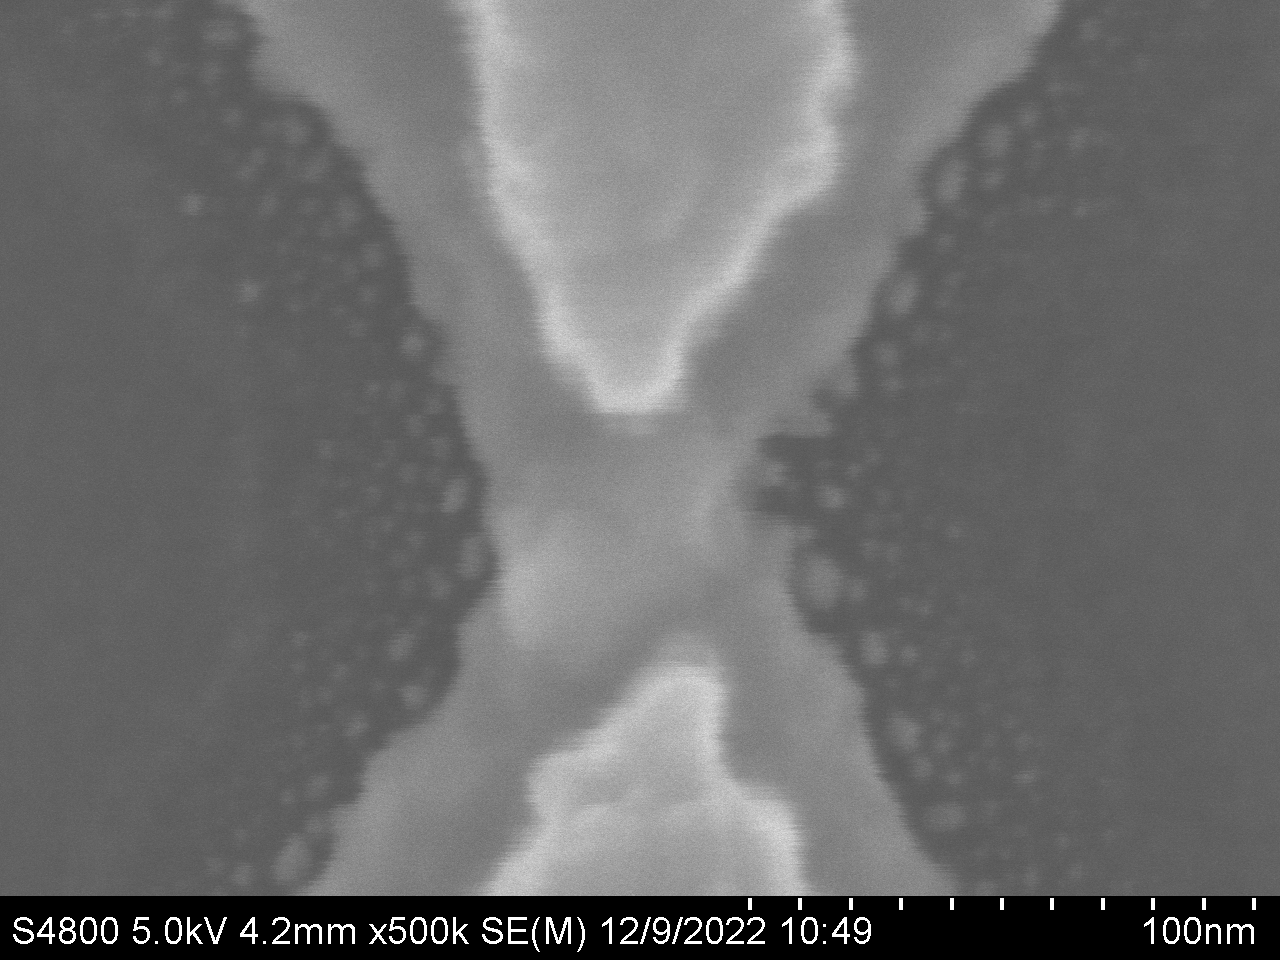
\includegraphics[width=0.32\textwidth]{Appendix_A/A3/A1.png}
         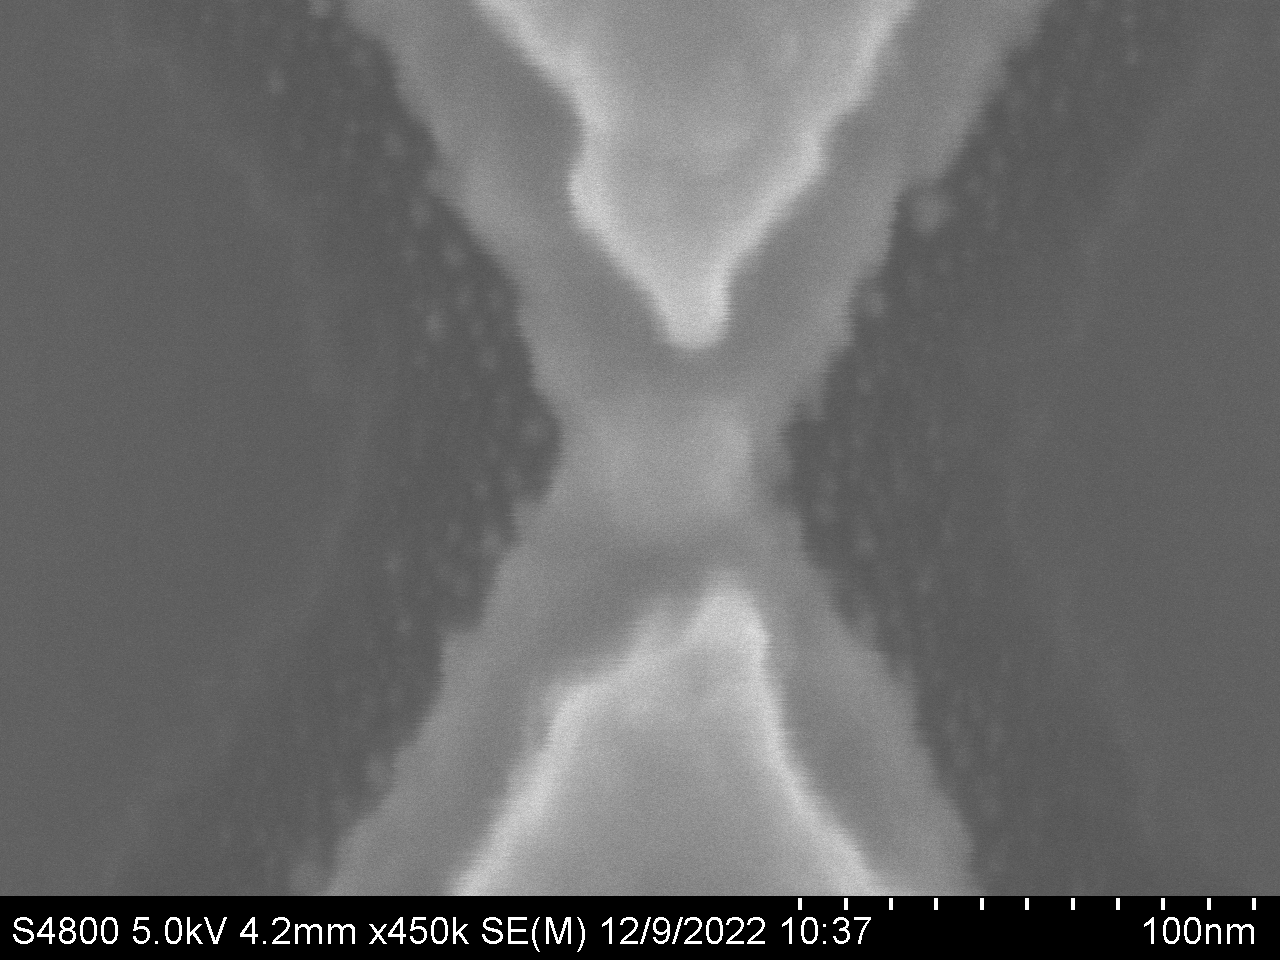
\includegraphics[width=0.32\textwidth]{Appendix_A/A3/A1_Alternate_contrast.png}
         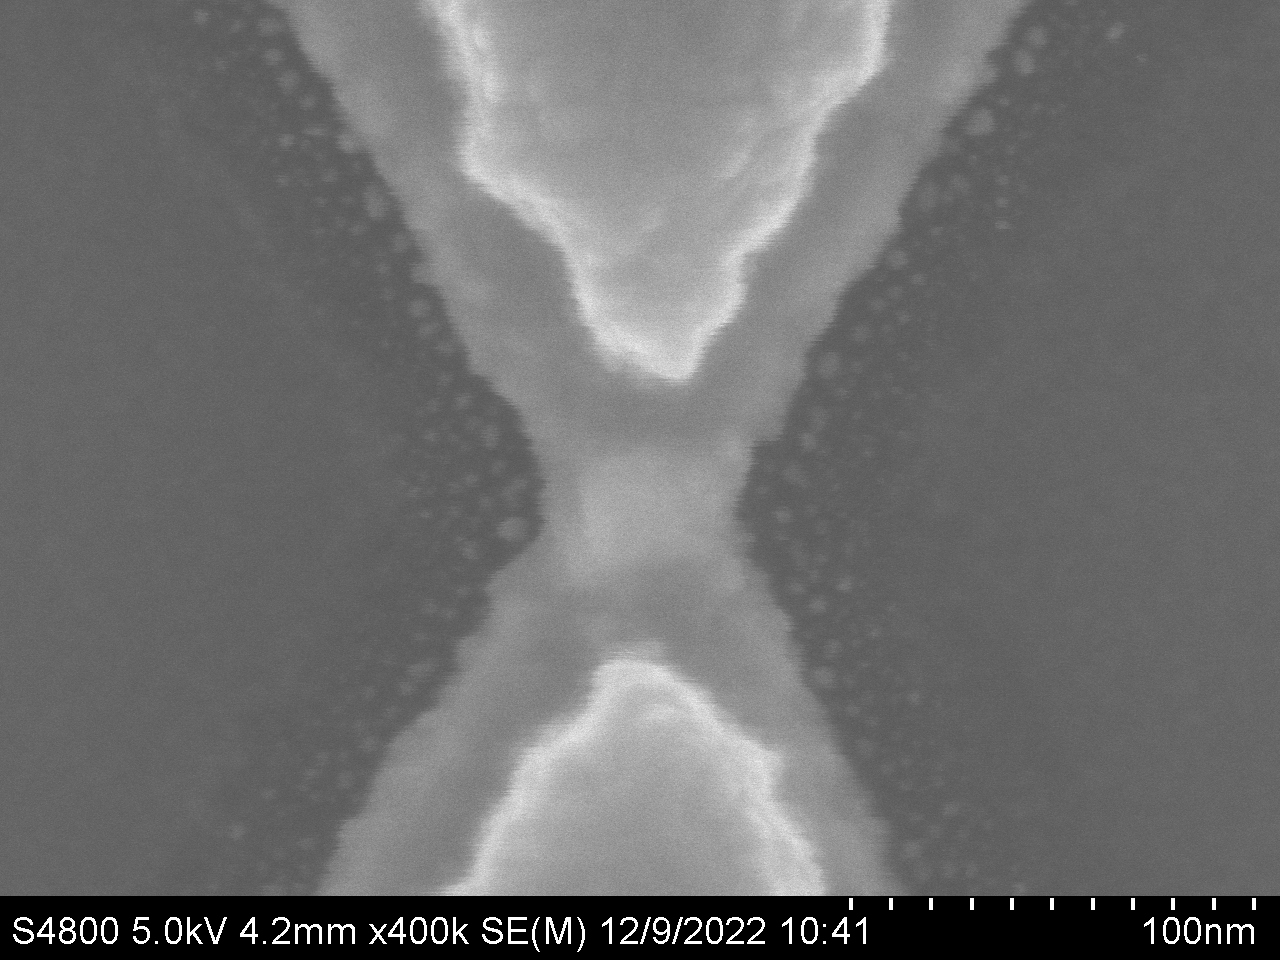
\includegraphics[width=0.32\textwidth]{Appendix_A/A3/A2.png}
         %\caption{A portion of the resist is irradiated with an electron beam in as specified pattern.}
         %\label{c}
     \end{subfigure}
     %\hfill
     \begin{subfigure}[b]{\textwidth}
         \centering
         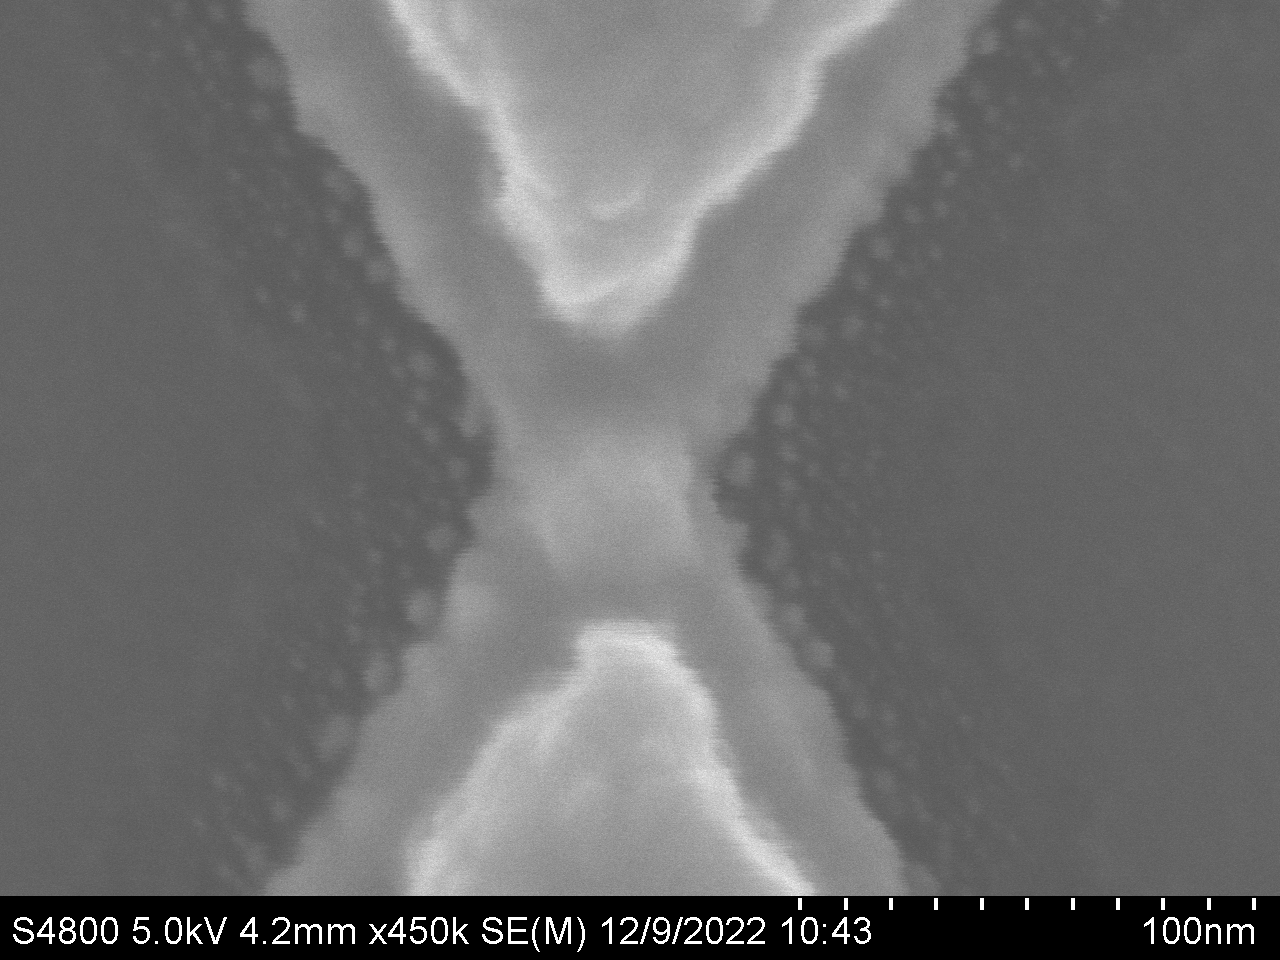
\includegraphics[width=0.32\textwidth]{Appendix_A/A3/A3.png}
         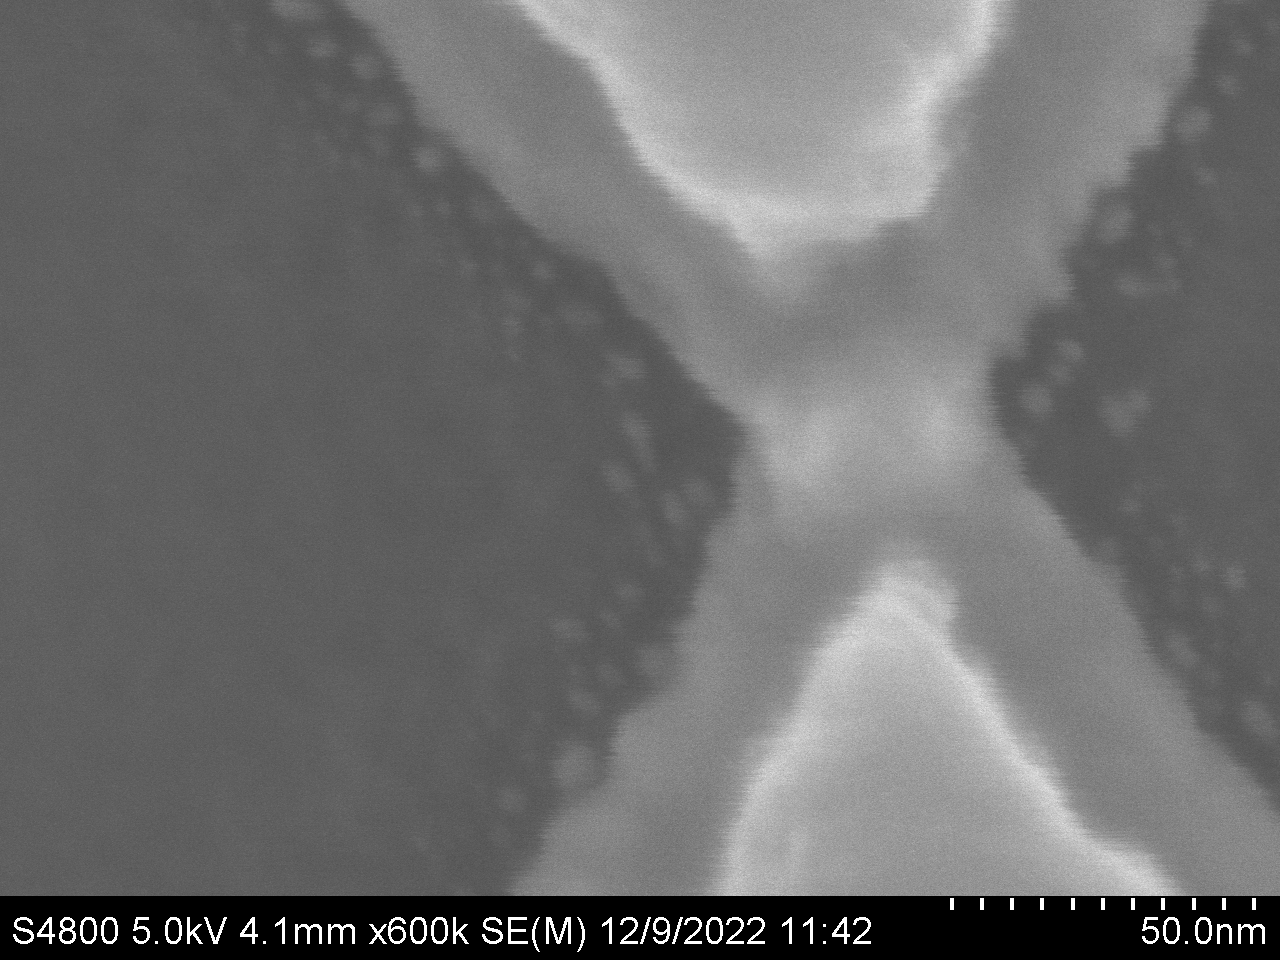
\includegraphics[width=0.32\textwidth]{Appendix_A/A3/B2_zoom.png}
         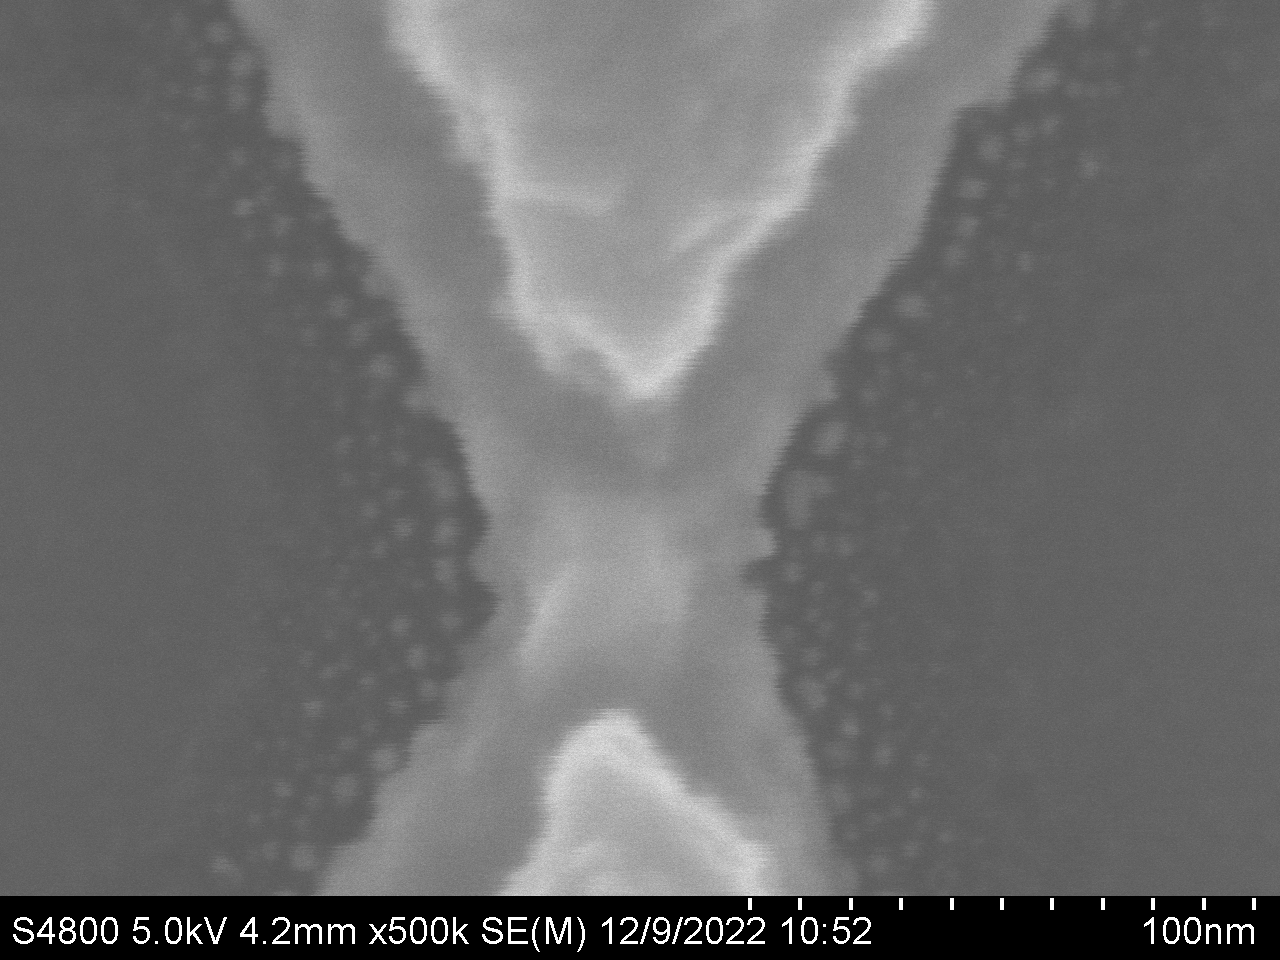
\includegraphics[width=0.32\textwidth]{Appendix_A/A3/A2_2.png}

         %\caption{A portion of the resist is irradiated with an electron beam in as specified pattern.}
         %\label{c}
     \end{subfigure}
        \caption{SEM images of AuNb devices with a 50 nm niobium layer.}
        \label{fig:}
        
\end{figure}

\subsubsection*{A4: AuNb, 60 nm Spacing}
\begin{figure}[H]
     \centering
     \begin{subfigure}[b]{\textwidth}
         \centering
         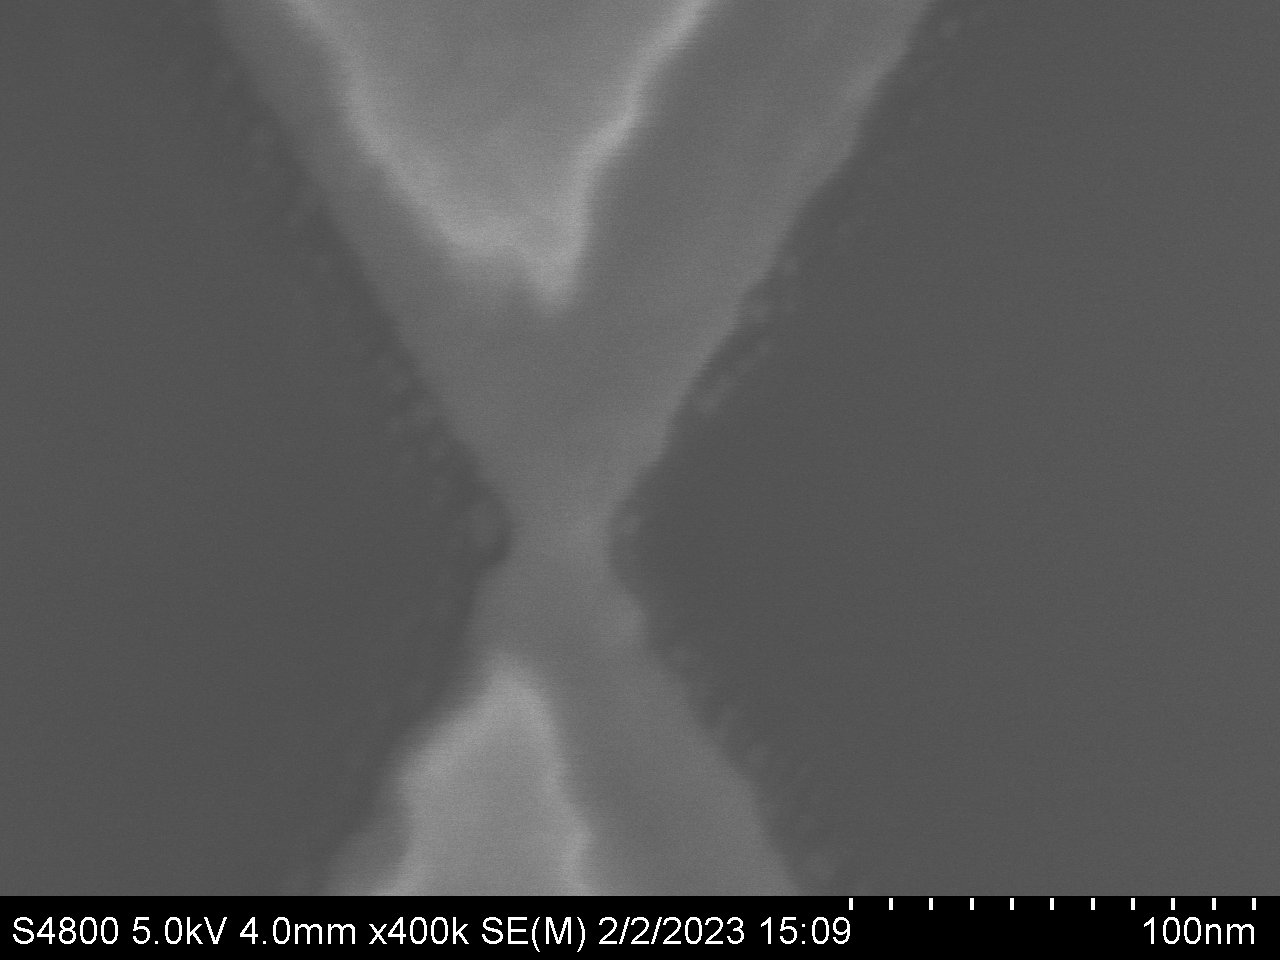
\includegraphics[width=0.32\textwidth]{Appendix_A/A4/60nmsetE1.png}
         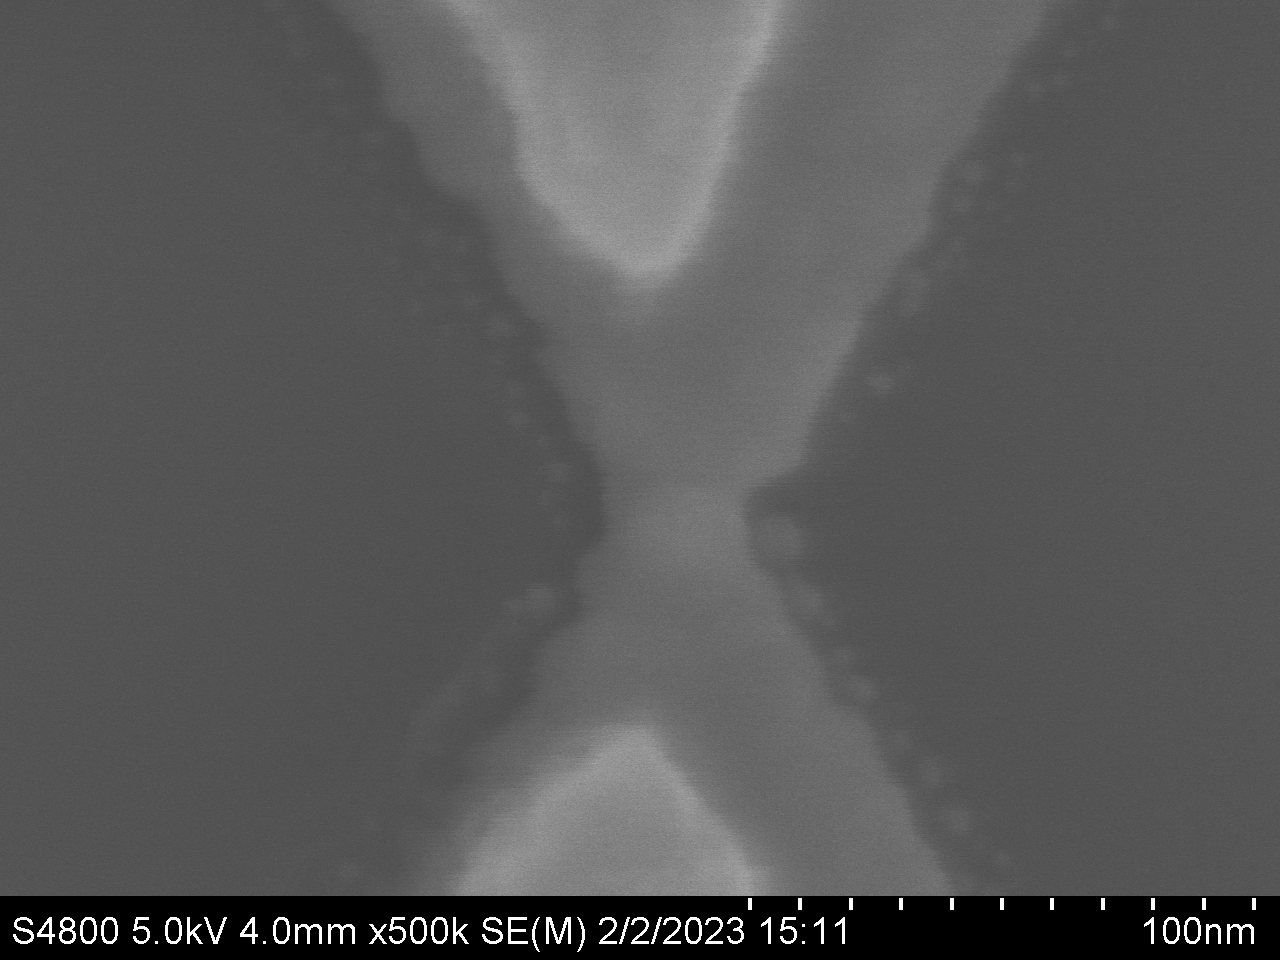
\includegraphics[width=0.32\textwidth]{Appendix_A/A4/60nmsetE2.png}
         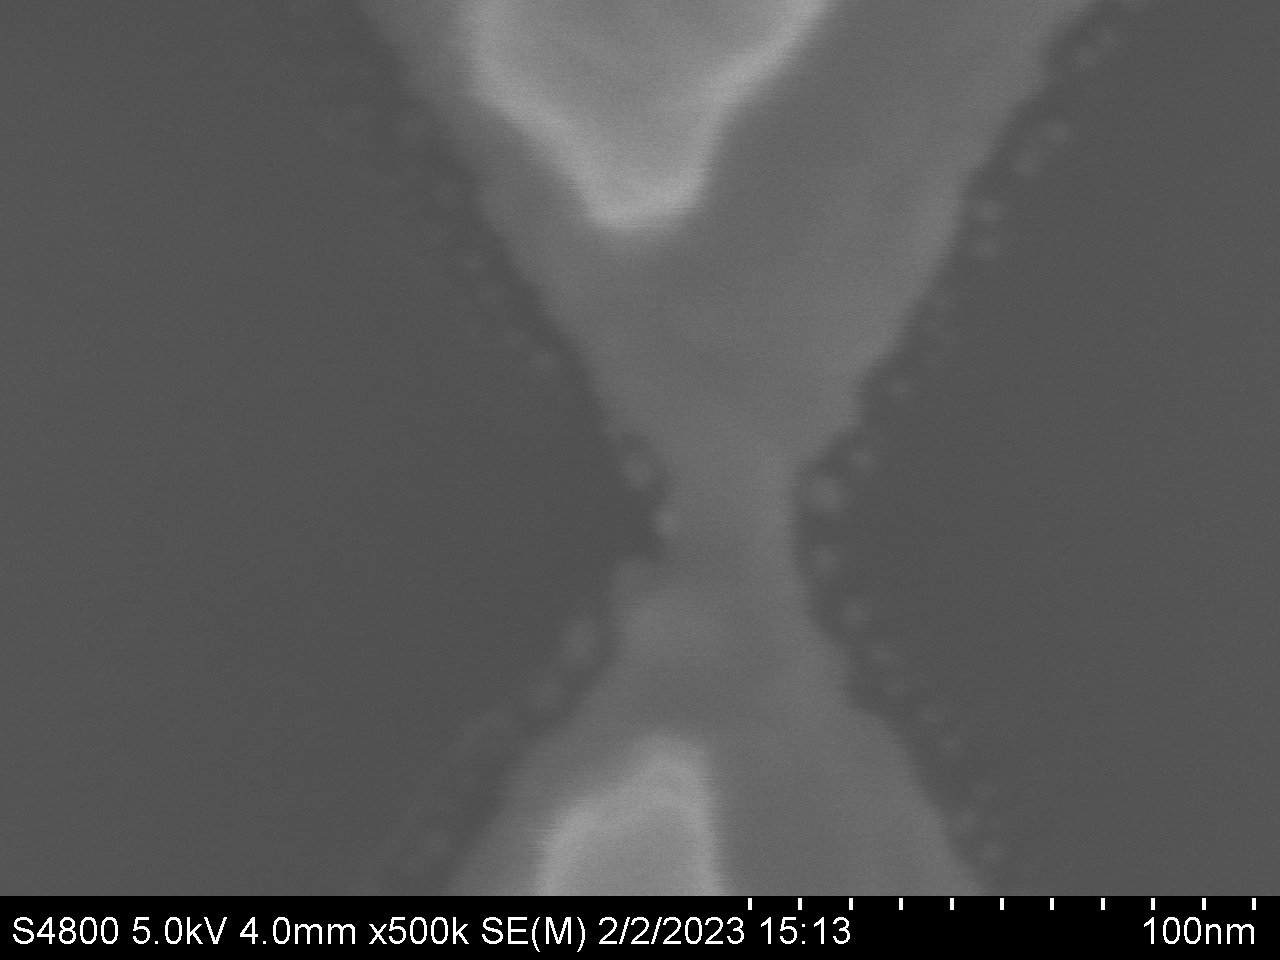
\includegraphics[width=0.32\textwidth]{Appendix_A/A4/60nmsetE3.png}
         %\caption{A portion of the resist is irradiated with an electron beam in as specified pattern.}
         %\label{c}
     \end{subfigure}
     %\hfill
     \begin{subfigure}[b]{\textwidth}
         \centering
         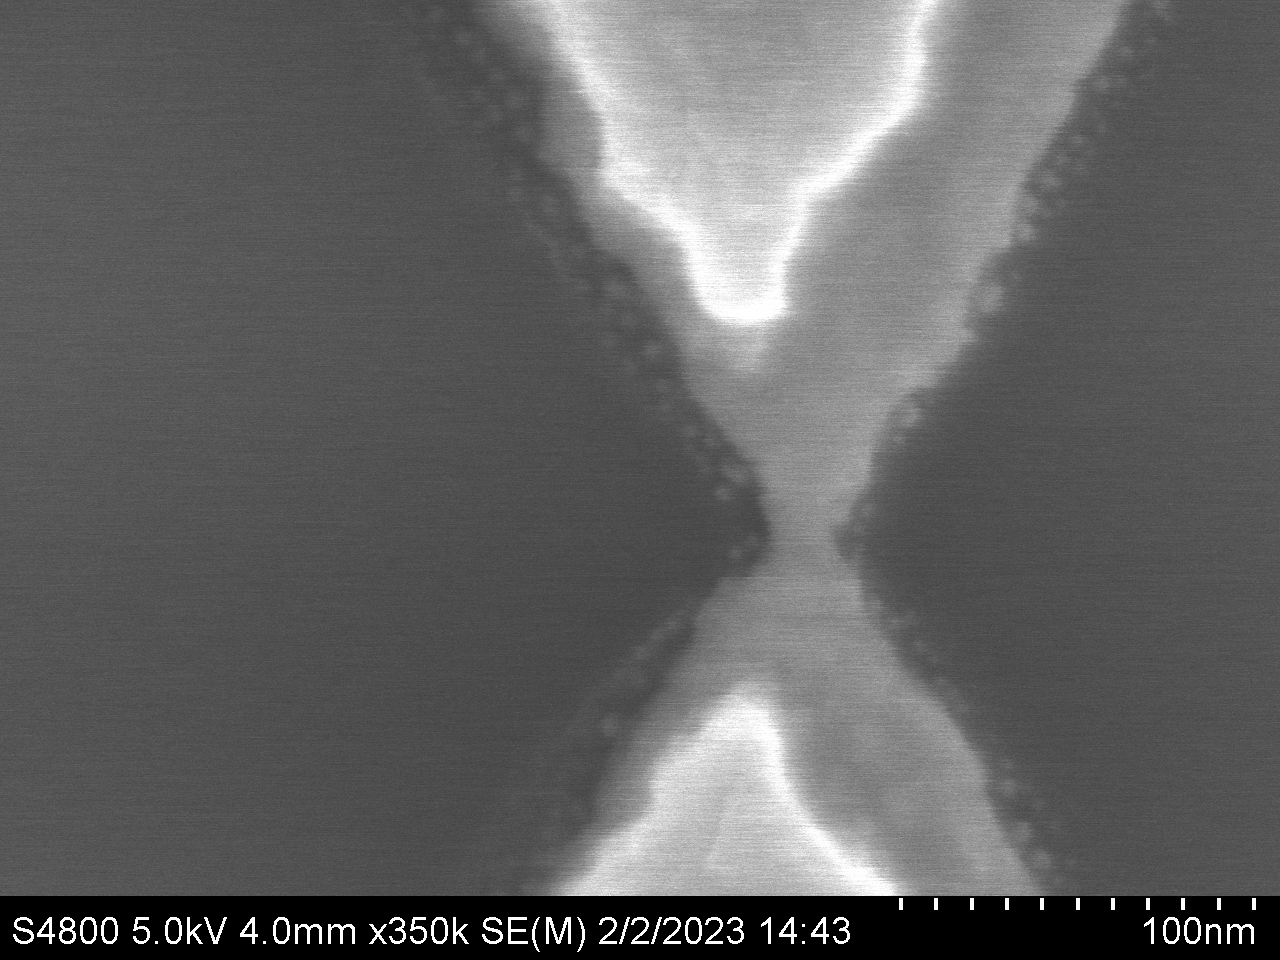
\includegraphics[width=0.32\textwidth]{Appendix_A/A4/variousb360nm.png}
         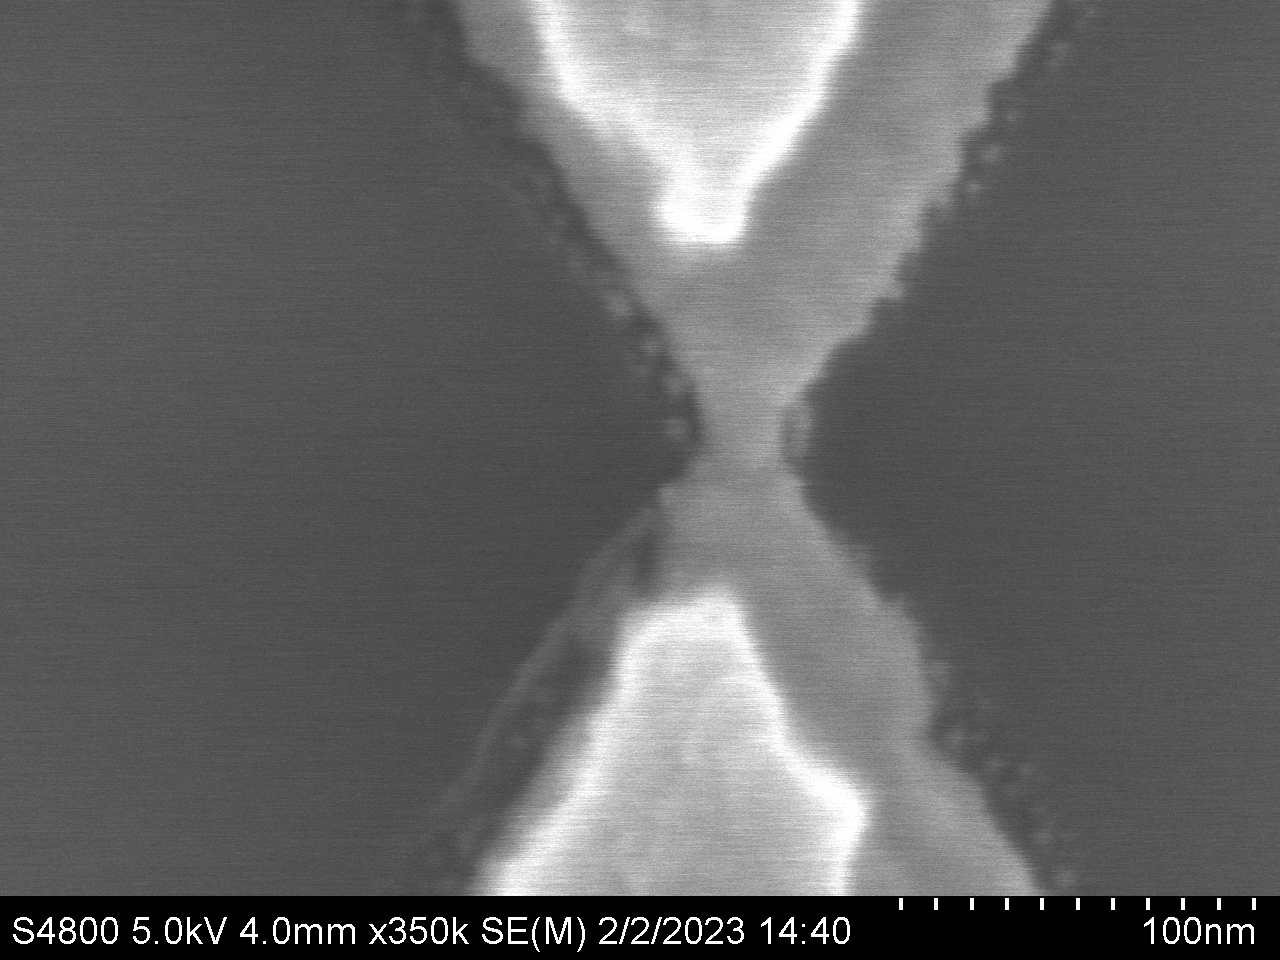
\includegraphics[width=0.32\textwidth]{Appendix_A/A4/variousB160nm.png}
         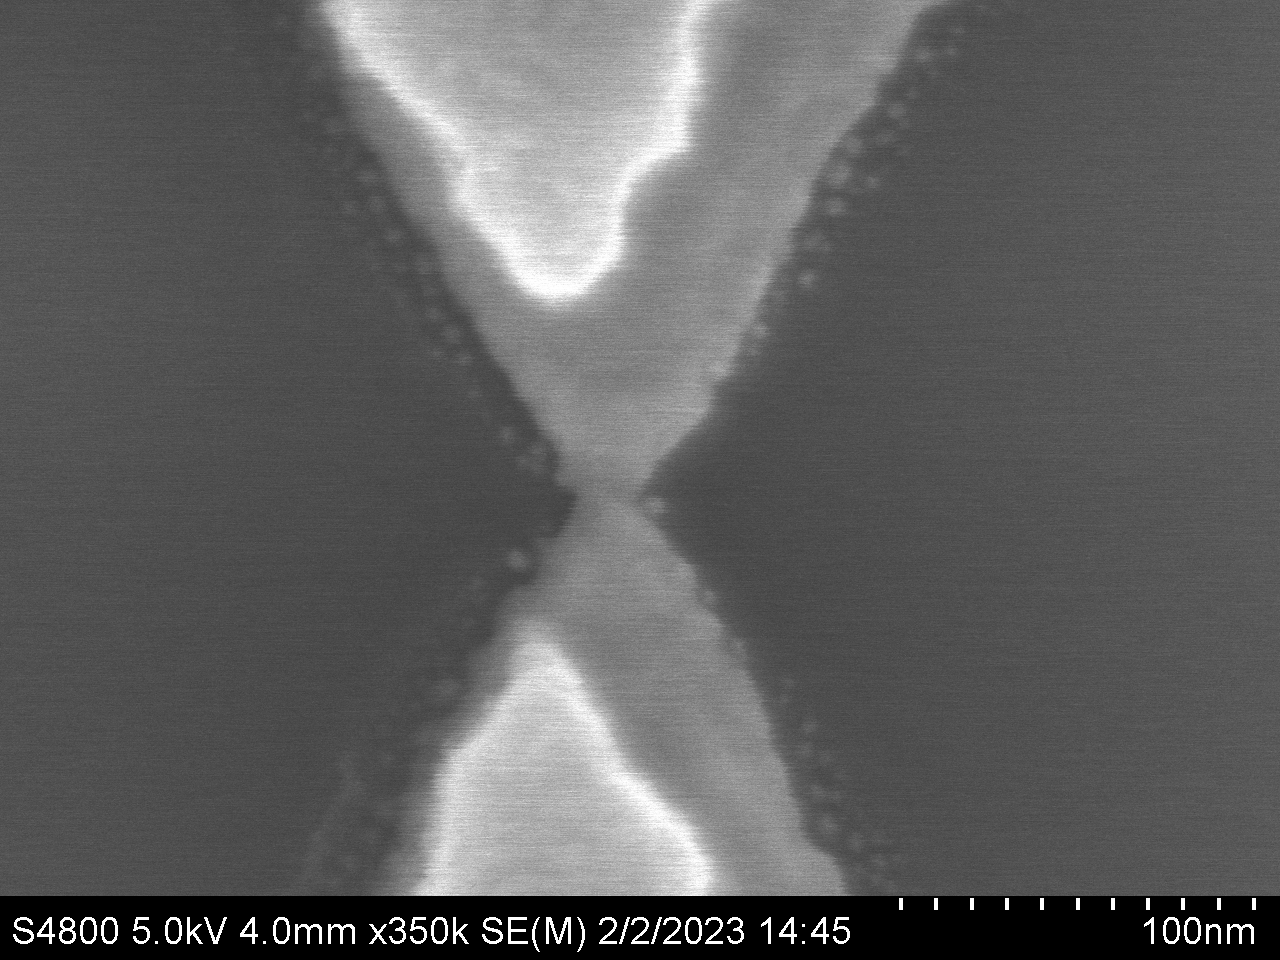
\includegraphics[width=0.32\textwidth]{Appendix_A/A4/variousb460nm.png}
         %\caption{A portion of the resist is irradiated with an electron beam in as specified pattern.}
         %\label{c}
     \end{subfigure}
        \caption{SEM images of AuNb devices with 60 nm spacing.}
        \label{fig:}
        
\end{figure}

\subsection{B: VI Measurement Results}
\subsubsection*{B1: PdNb}

\begin{figure}[H]
     \centering
     \begin{subfigure}[b]{\textwidth}
         \centering
         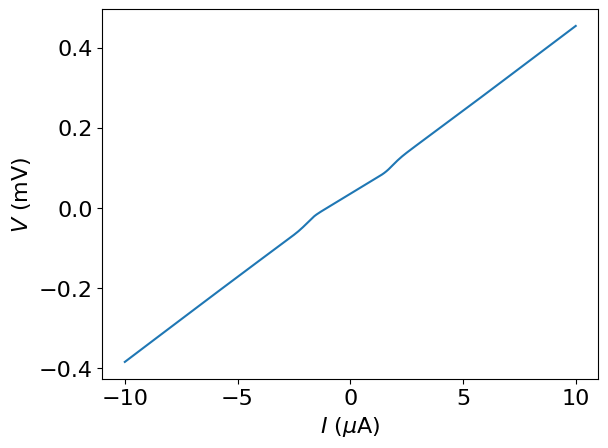
\includegraphics[width=0.32\textwidth]{Appendix_B/B1/VI_PdNb_numid2.png}
         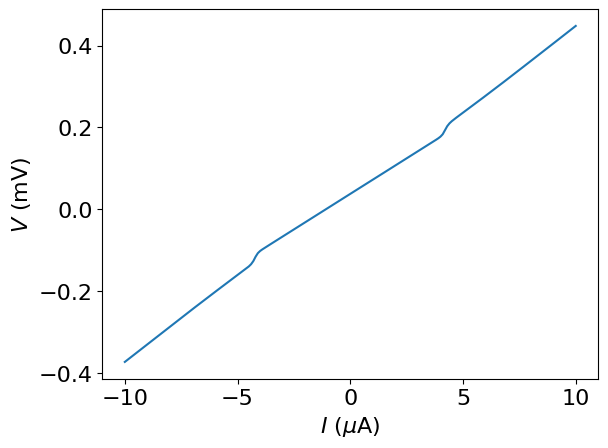
\includegraphics[width=0.32\textwidth]{Appendix_B/B1/VI_PdNb_numid3.png}
         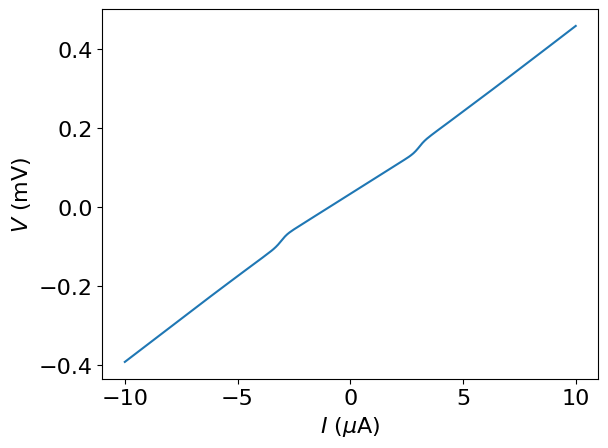
\includegraphics[width=0.32\textwidth]{Appendix_B/B1/VI_PdNb_numid4.png}
         %\caption{A portion of the resist is irradiated with an electron beam in as specified pattern.}
         %\label{c}
     \end{subfigure}
     %\hfill
     \begin{subfigure}[b]{\textwidth}
         \centering
         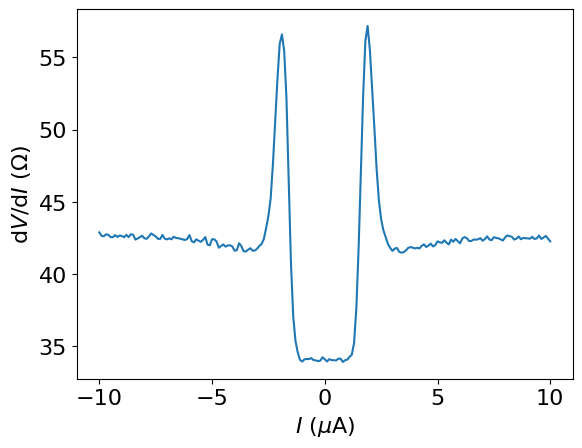
\includegraphics[width=0.32\textwidth]{Appendix_B/B1/dVdI_PdNb_numid2.png}
         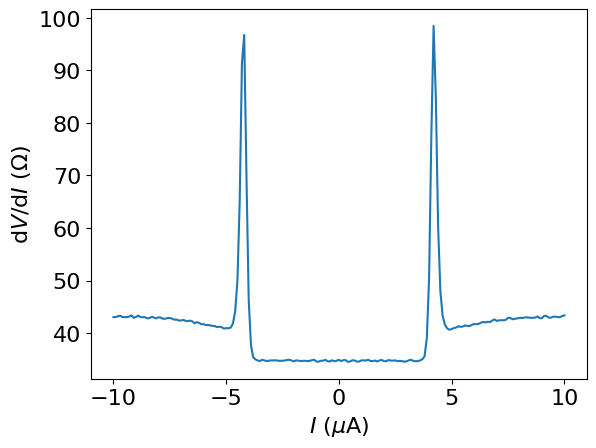
\includegraphics[width=0.32\textwidth]{Appendix_B/B1/dVdI_PdNb_numid3.png}
         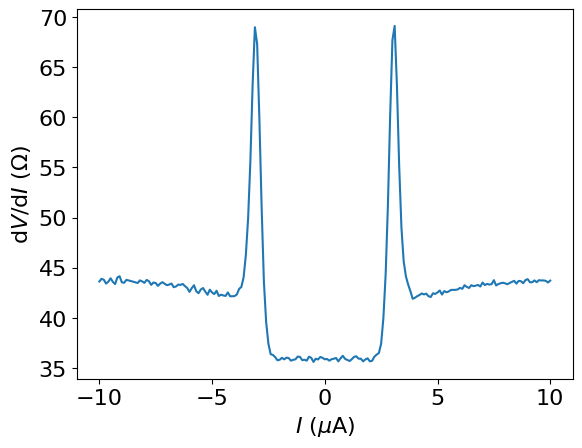
\includegraphics[width=0.32\textwidth]{Appendix_B/B1/dVdI_PdNb_numid4.png}
         %\caption{A portion of the resist is irradiated with an electron beam in as specified pattern.}
         %\label{c}
     \end{subfigure}
        \caption{VI measurements and their derivatives, measured at 1.2 K}
        \label{fig:}
        
\end{figure}

\subsubsection*{B2: AuNb, 100 nm Nb}

\begin{figure}[H]
     \centering
     \begin{subfigure}[b]{\textwidth}
         \centering
         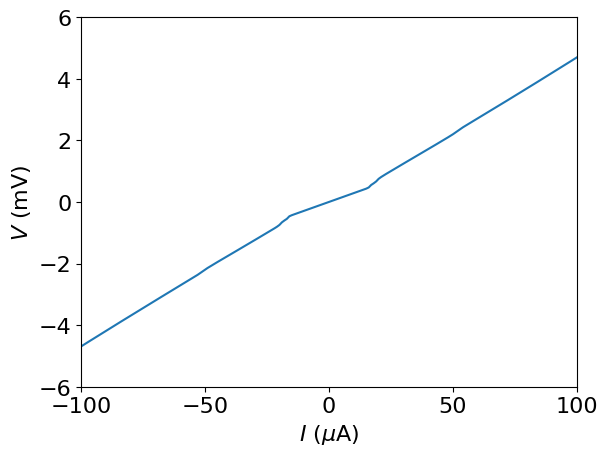
\includegraphics[width=0.32\textwidth]{Appendix_B/B2/VI_AuNbV2_numid19.png}
         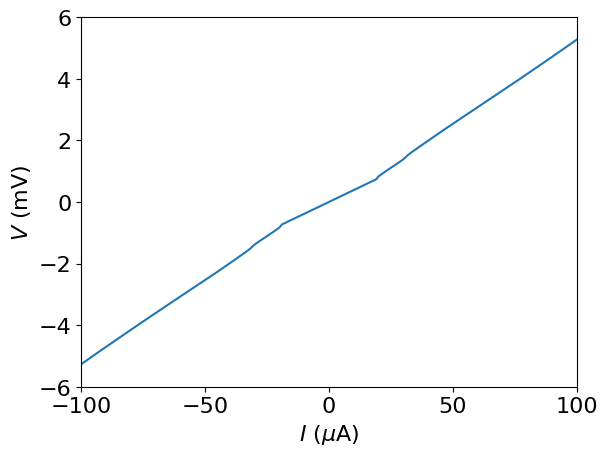
\includegraphics[width=0.32\textwidth]{Appendix_B/B2/VI_AuNbV2_numid20.png}
         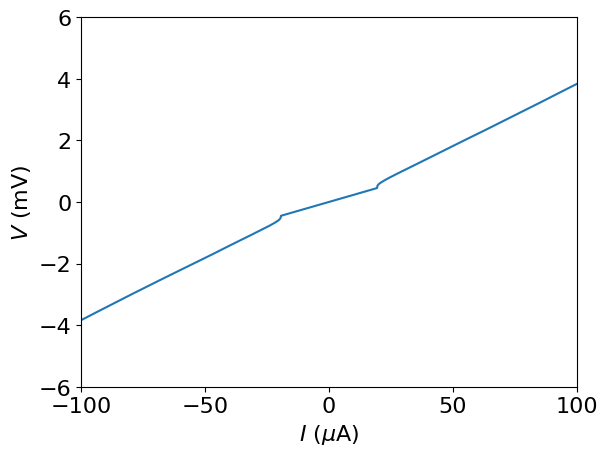
\includegraphics[width=0.32\textwidth]{Appendix_B/B2/VI_AuNbV2_numid26.png}
         %\caption{A portion of the resist is irradiated with an electron beam in as specified pattern.}
         %\label{c}
     \end{subfigure}
     %\hfill
     \begin{subfigure}[b]{\textwidth}
         \centering
         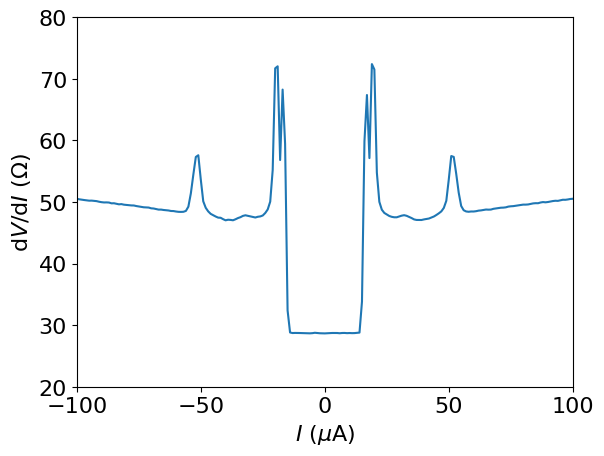
\includegraphics[width=0.32\textwidth]{Appendix_B/B2/dVdI_AuNbV2_numid19.png}
         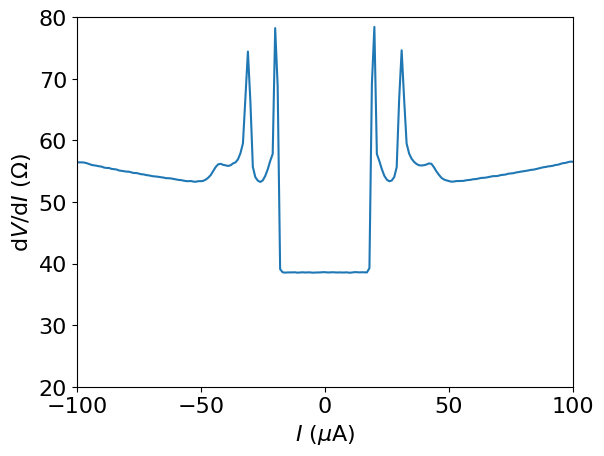
\includegraphics[width=0.32\textwidth]{Appendix_B/B2/dVdI_AuNbV2_numid20.png}
         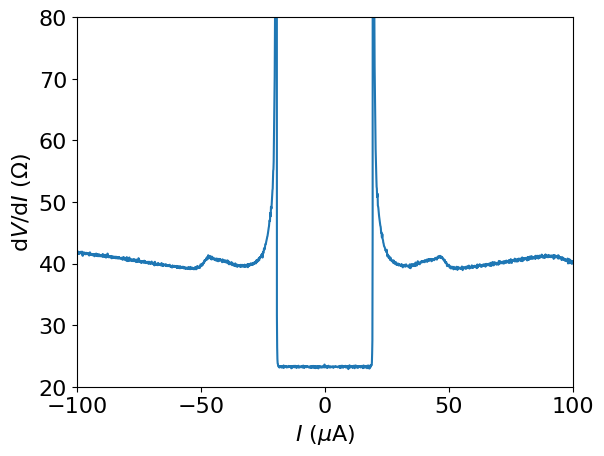
\includegraphics[width=0.32\textwidth]{Appendix_B/B2/dVdI_AuNbV2_numid26.png}
         %\caption{A portion of the resist is irradiated with an electron beam in as specified pattern.}
         %\label{c}
     \end{subfigure}
        \caption{VI measurements and their derivatives, measured at 1.8 K}
        \label{fig:}
        
\end{figure}

\subsubsection*{B3: AuNb, 50 nm Nb}

\begin{figure}[H]
     \centering
     \begin{subfigure}[b]{\textwidth}
         \centering
         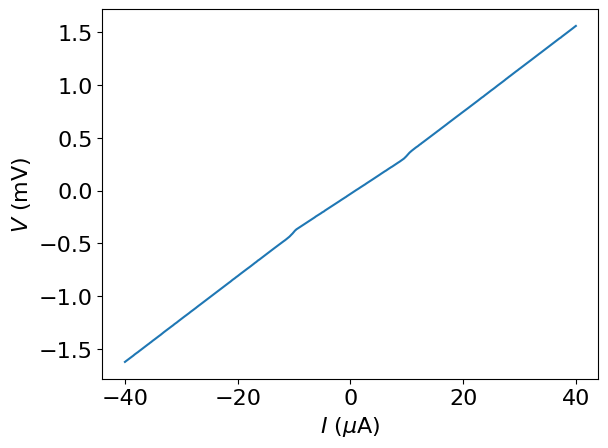
\includegraphics[width=0.32\textwidth]{Appendix_B/B3/VI_AuNbV3DF_numid12.png}
         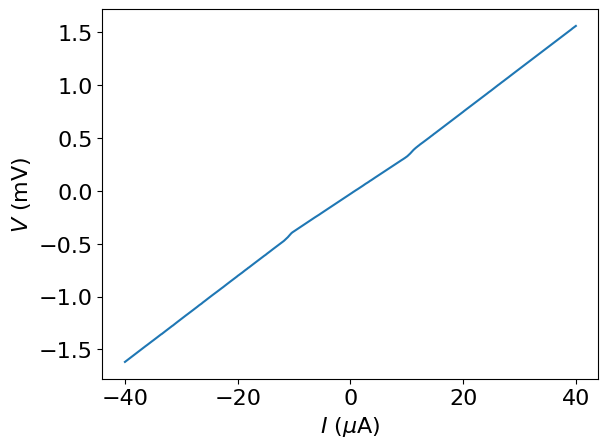
\includegraphics[width=0.32\textwidth]{Appendix_B/B3/VI_AuNbV3DF_numid13.png}
         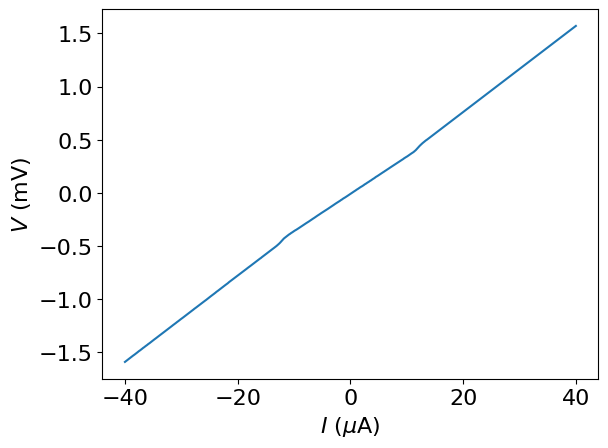
\includegraphics[width=0.32\textwidth]{Appendix_B/B3/VI_AuNbV3DF_numid14.png}
         %\caption{A portion of the resist is irradiated with an electron beam in as specified pattern.}
         %\label{c}
     \end{subfigure}
     %\hfill
     \begin{subfigure}[b]{\textwidth}
         \centering
         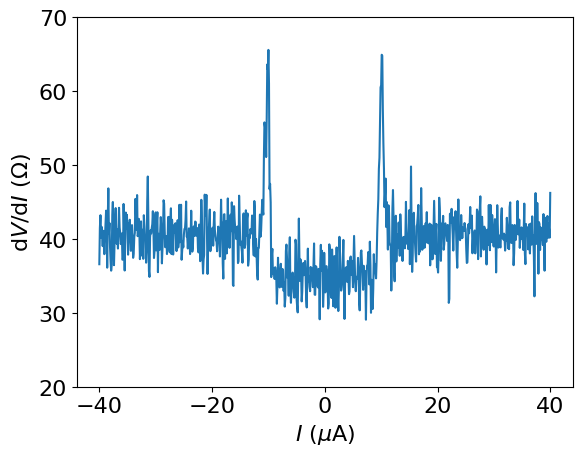
\includegraphics[width=0.32\textwidth]{Appendix_B/B3/dVdI_AuNbV3DF_numid12.png}
         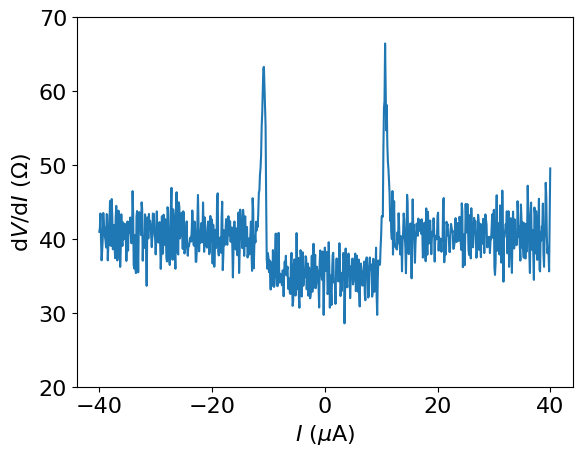
\includegraphics[width=0.32\textwidth]{Appendix_B/B3/dVdI_AuNbV3DF_numid13.png}
         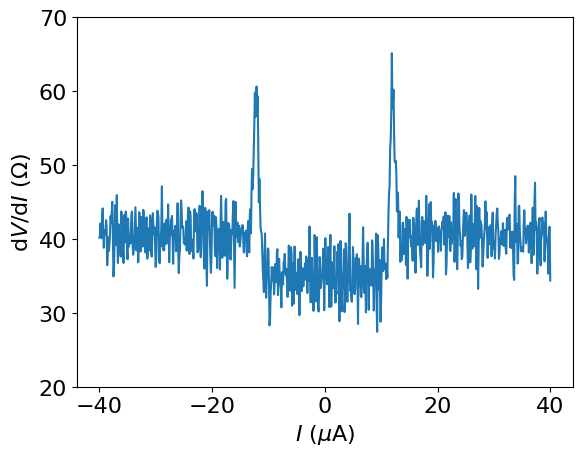
\includegraphics[width=0.32\textwidth]{Appendix_B/B3/dVdI_AuNbV3DF_numid14.png}
         %\caption{A portion of the resist is irradiated with an electron beam in as specified pattern.}
         %\label{c}
     \end{subfigure}
        \caption{VI measurements and their derivatives. The four figures on the left have been measured at 1.9 K, the two on the right at 40 mK.}
        \label{fig:}
        
\end{figure}


\subsubsection*{B4: AuNb, 60 nm Spacing}
\begin{figure}[H]
     \centering
     \begin{subfigure}[b]{\textwidth}
         \centering
         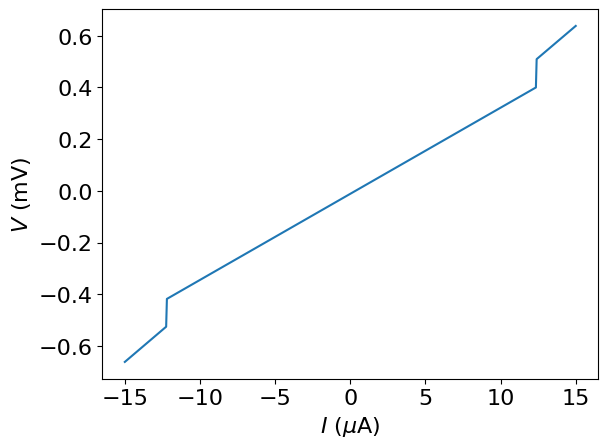
\includegraphics[width=0.32\textwidth]{Appendix_B/B4/VI_AuNb60nm_numid36.png}
         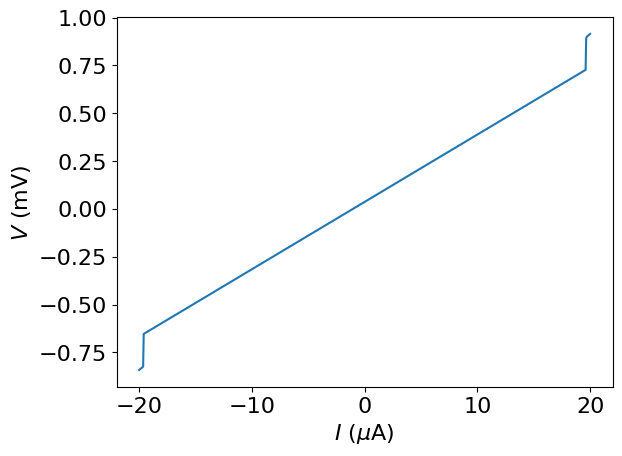
\includegraphics[width=0.32\textwidth]{Appendix_B/B4/VI_AuNb60nm_numid38.png}
         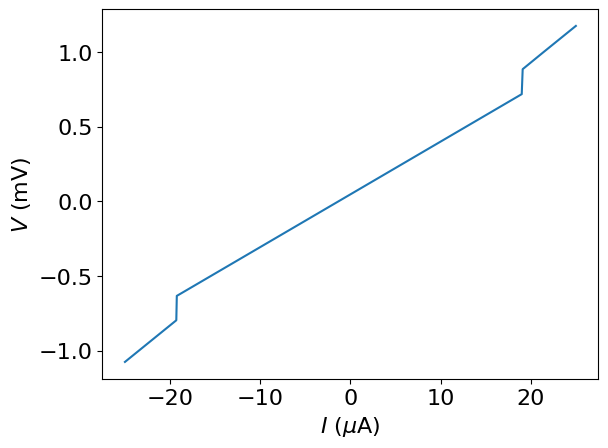
\includegraphics[width=0.32\textwidth]{Appendix_B/B4/VI_AuNb60nm_numid40.png}
         %\caption{A portion of the resist is irradiated with an electron beam in as specified pattern.}
         %\label{c}
     \end{subfigure}
     %\hfill
     \begin{subfigure}[b]{\textwidth}
         \centering
         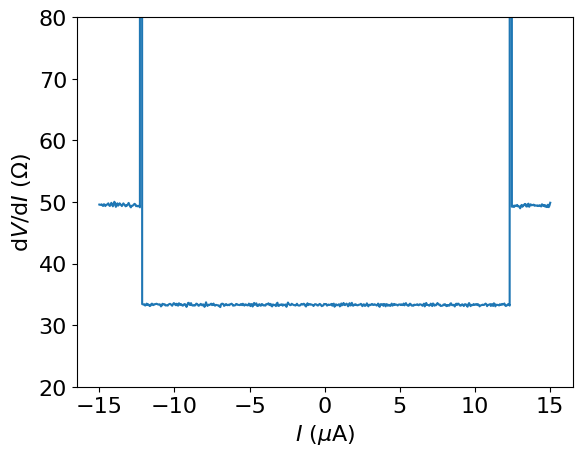
\includegraphics[width=0.32\textwidth]{Appendix_B/B4/dVdI_AuNb60nm_numid36.png}
         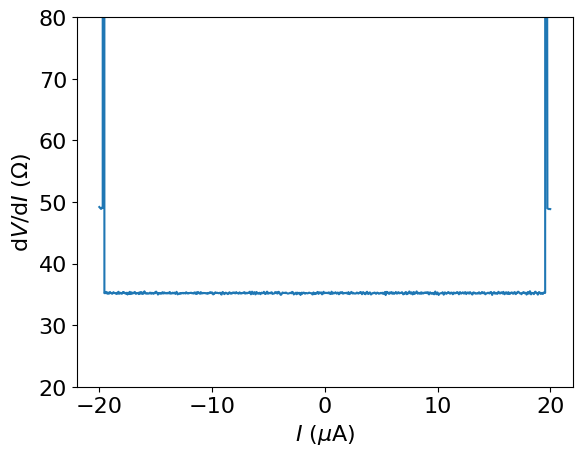
\includegraphics[width=0.32\textwidth]{Appendix_B/B4/dVdI_AuNb60nm_numid38.png}
         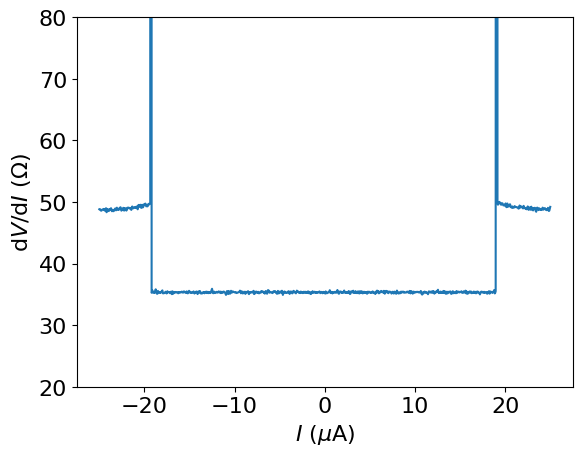
\includegraphics[width=0.32\textwidth]{Appendix_B/B4/dVdI_AuNb60nm_numid40.png}
         %\caption{A portion of the resist is irradiated with an electron beam in as specified pattern.}
         %\label{c}
     \end{subfigure}
        \caption{VI measurements and their derivatives, measured at 30 mK. Current has been swept from 0 in the positive direction, and then from 0 in the negative direction.}
        \label{fig:}
        
\end{figure}


\subsection{C: VIT Measurement Results}
\subsubsection*{C1: PdNb}
\begin{figure}[H]
     \centering
     \begin{subfigure}[b]{\textwidth}
         \centering
         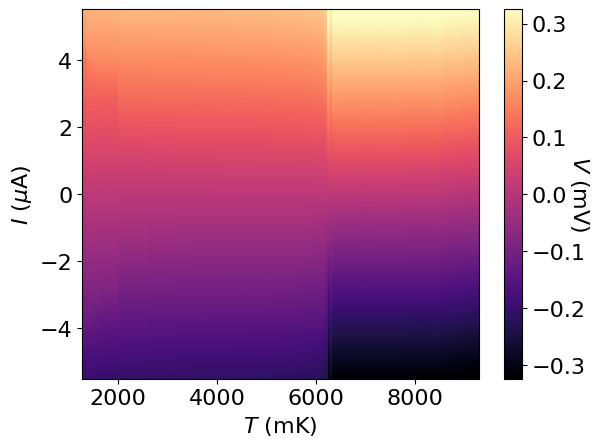
\includegraphics[width=0.32\textwidth]{Appendix_C/C1/PdNb_VIT.png}
         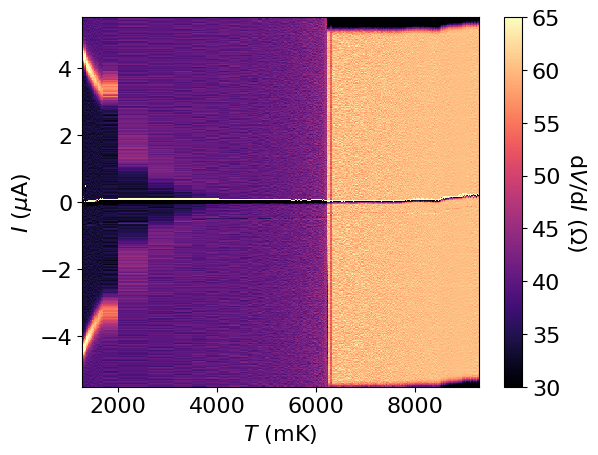
\includegraphics[width=0.32\textwidth]{Appendix_C/C1/PdNb_dVdIT.png}
         %\caption{A portion of the resist is irradiated with an electron beam in as specified pattern.}
         %\label{c}
     \end{subfigure}
        \caption{VIT measurement.}
        \label{fig:}
        
\end{figure}

\subsubsection*{C2: AuNb, 100 nm Nb}
\begin{figure}[H]
     \centering
     \begin{subfigure}[b]{\textwidth}
         \centering
         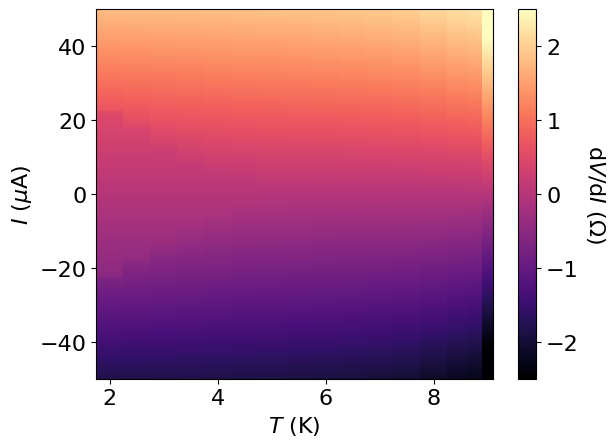
\includegraphics[width=0.32\textwidth]{Appendix_C/C2/AuNbV2_VIT.png}
         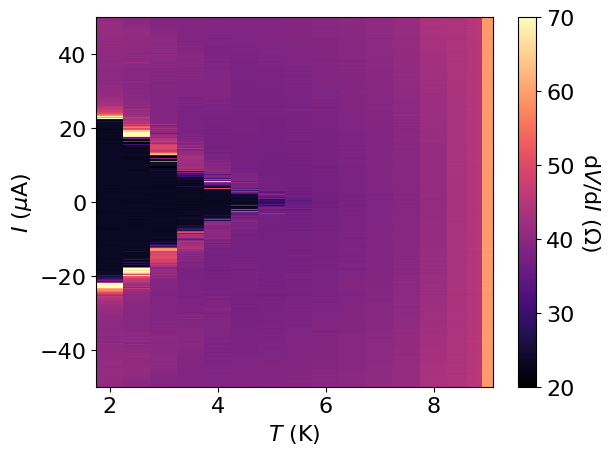
\includegraphics[width=0.32\textwidth]{Appendix_C/C2/AuNbV2_dVdIT.png}
         %\caption{A portion of the resist is irradiated with an electron beam in as specified pattern.}
         %\label{c}
     \end{subfigure}
        \caption{VIT measurement.}
        \label{fig:}
        
\end{figure}

\subsubsection*{C3: AuNb, 50 nm Nb}

\begin{figure}[H]
     \centering
     \begin{subfigure}[b]{\textwidth}
         \centering
         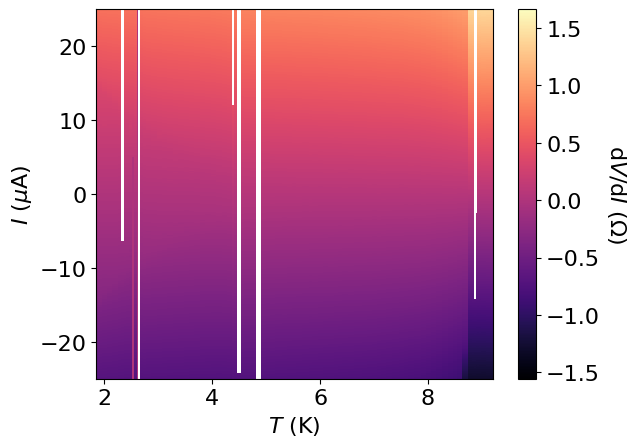
\includegraphics[width=0.32\textwidth]{Appendix_C/C3/AuNbV3_VIT.png}
         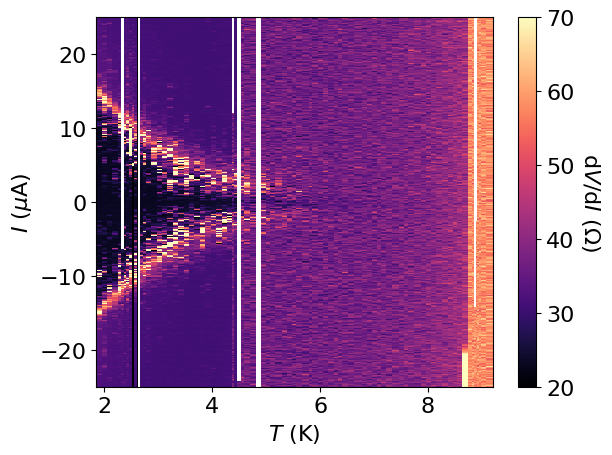
\includegraphics[width=0.32\textwidth]{Appendix_C/C3/AuNbV3_dVdIT.png}
         %\caption{A portion of the resist is irradiated with an electron beam in as specified pattern.}
         %\label{c}
     \end{subfigure}
     %\hfill
     \begin{subfigure}[b]{\textwidth}
         \centering
         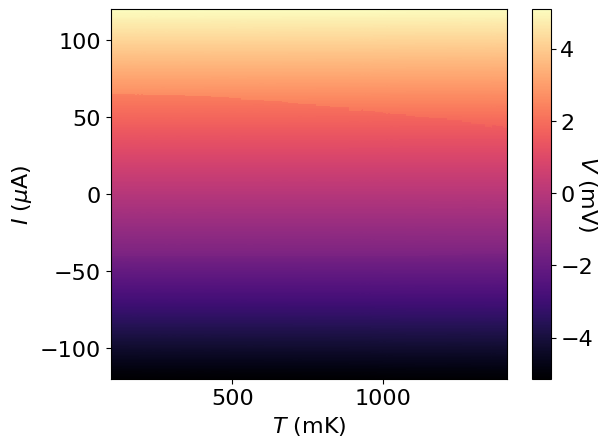
\includegraphics[width=0.32\textwidth]{Appendix_C/C3/AuNbV3DF_VIT.png}
         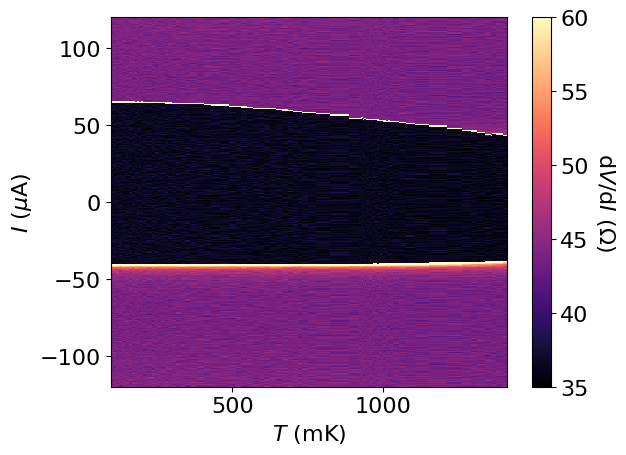
\includegraphics[width=0.32\textwidth]{Appendix_C/C3/AuNbV3DF_dVdIT.png}
         %\caption{A portion of the resist is irradiated with an electron beam in as specified pattern.}
         %\label{c}
     \end{subfigure}
        \caption{VIT measurements. Top: Dip-Stick, higher T range. Bottom: Dilution Fridge, lower T range. Different devices made with the same fabrication parameters.}
        \label{fig:}
        
\end{figure}

\subsubsection*{C4: AuNb, 60 nm Spacing}
\begin{figure}[H]
     \centering
     \begin{subfigure}[b]{\textwidth}
         \centering
         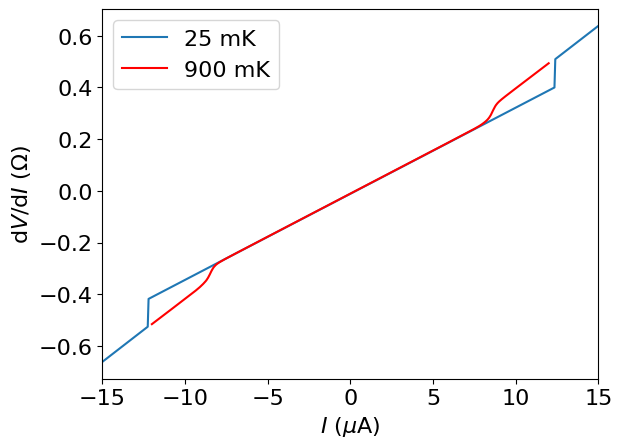
\includegraphics[width=0.32\textwidth]{Appendix_C/C4/AuNb60nm_VIT_A1.png}
         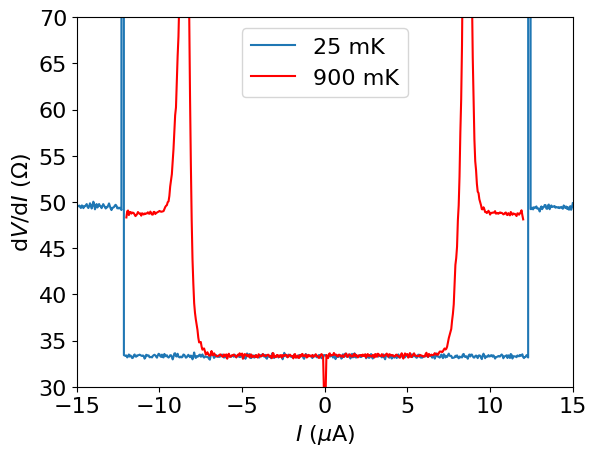
\includegraphics[width=0.32\textwidth]{Appendix_C/C4/AuNb60nm_dVdIT_A1.png}
         %\caption{A portion of the resist is irradiated with an electron beam in as specified pattern.}
         %\label{c}
     \end{subfigure}
     %\hfill
     \begin{subfigure}[b]{\textwidth}
         \centering
         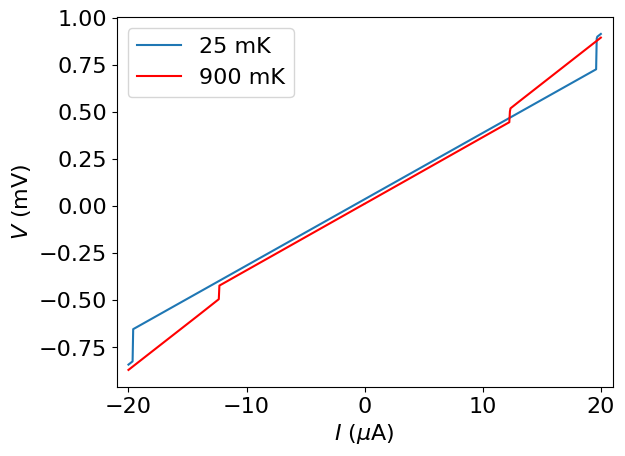
\includegraphics[width=0.32\textwidth]{Appendix_C/C4/AuNb60nm_VIT_A6.png}
         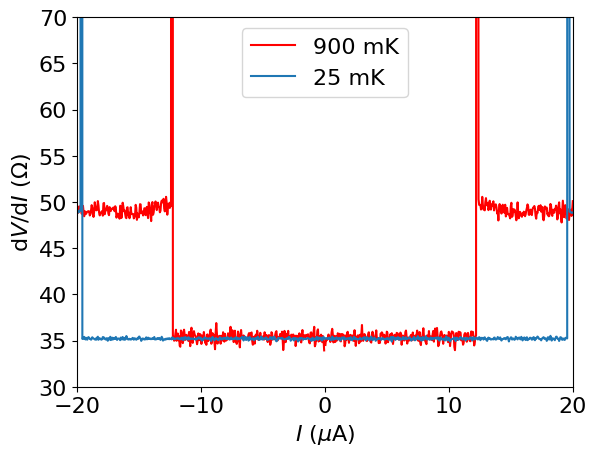
\includegraphics[width=0.32\textwidth]{Appendix_C/C4/AuNb60nm_dVdIT_A6.png}
         %\caption{A portion of the resist is irradiated with an electron beam in as specified pattern.}
         %\label{c}
     \end{subfigure}
        \caption{Two sets of VI measurements of the same device, taken at two different temperatures.}
        \label{fig:}

\end{figure}

\subsection{D: BVI Measurement Results}
\subsubsection*{D1: PdNb}
\subsubsection*{Z Direction, High Field}


\begin{figure}[H]
     \centering
     \begin{subfigure}[b]{\textwidth}
         \centering
         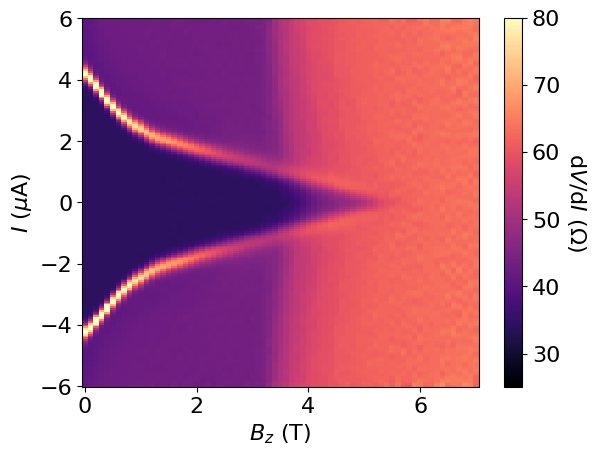
\includegraphics[width=0.32\textwidth]{dVdIBZ_36.png}
         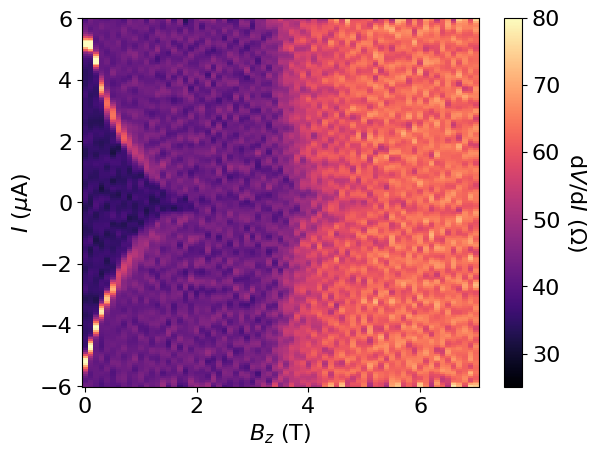
\includegraphics[width=0.32\textwidth]{dVdIBZ_43.png}
         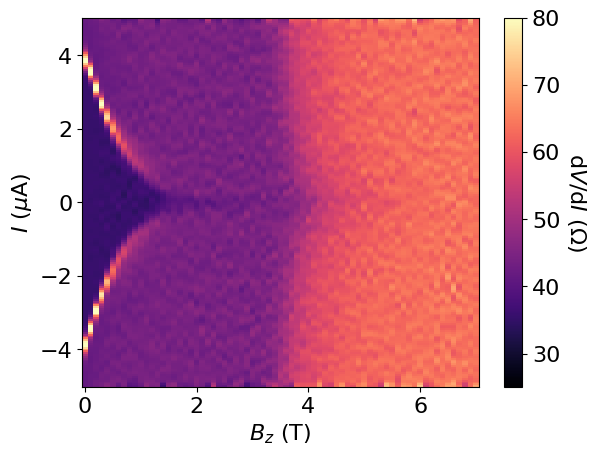
\includegraphics[width=0.32\textwidth]{dVdIBZ_57.png}
         %\caption{A portion of the resist is irradiated with an electron beam in as specified pattern.}
         %\label{c}
     \end{subfigure}
	 \caption{Out of plane BVI measurements.}
     \label{fig:}
        
\end{figure}

\subsubsection*{X,Y,Z directions, Low field}

\begin{figure}[H]
     \centering
     \begin{subfigure}[b]{\textwidth}
         \centering
         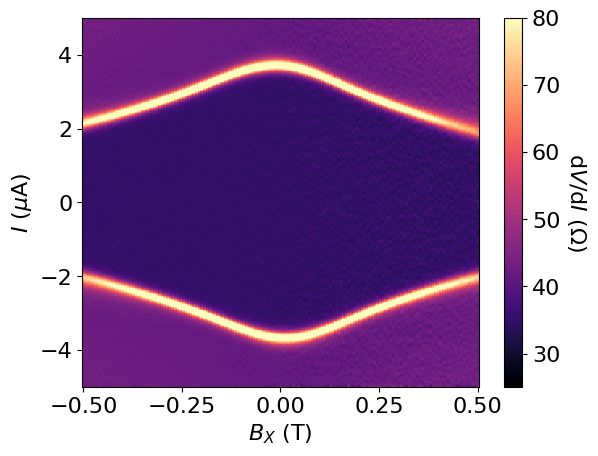
\includegraphics[width=0.32\textwidth]{dVdIBX_64.png}
         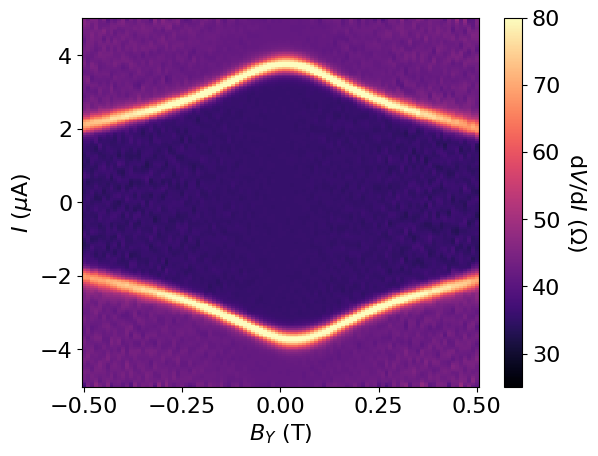
\includegraphics[width=0.32\textwidth]{dVdIBY_63.png}
         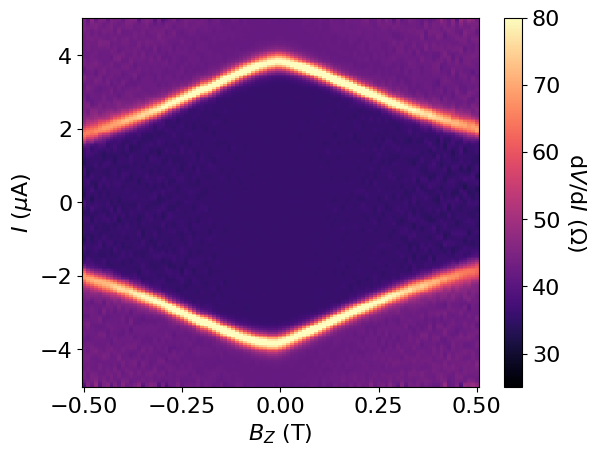
\includegraphics[width=0.32\textwidth]{dVdIBZ_61.png}
         %\caption{A portion of the resist is irradiated with an electron beam in as specified pattern.}
         %\label{c}
     \end{subfigure}
	 \caption{BVI measurements in the X, Y and Z directions.}
     \label{fig:}
        
\end{figure}

\subsubsection*{$\phi$, $\theta$ Sweep}

\begin{figure}[H]
     \centering
     \begin{subfigure}[b]{\textwidth}
         \centering
         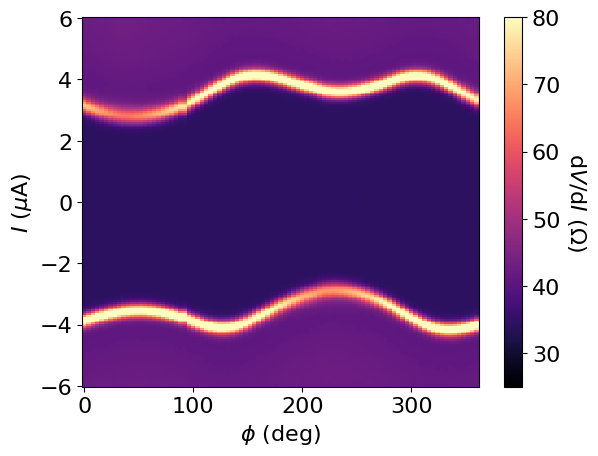
\includegraphics[width=0.32\textwidth]{dVdIphisweep_49.png}
         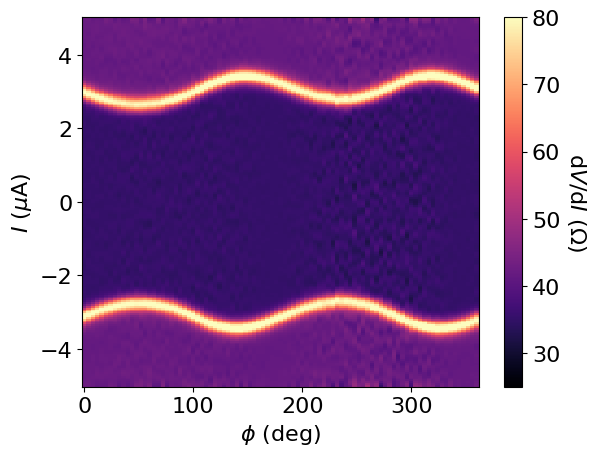
\includegraphics[width=0.32\textwidth]{dVdIphisweep_68.png}
         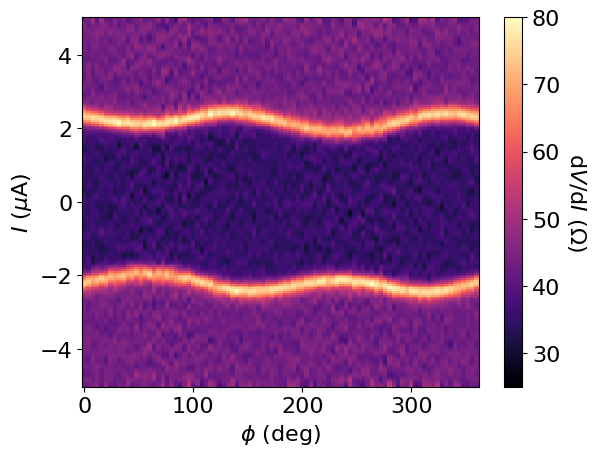
\includegraphics[width=0.32\textwidth]{dVdIphisweep_69.png}
         %\caption{A portion of the resist is irradiated with an electron beam in as specified pattern.}
         %\label{c}
     \end{subfigure}
     %\hfill
     \begin{subfigure}[b]{\textwidth}
         \centering
         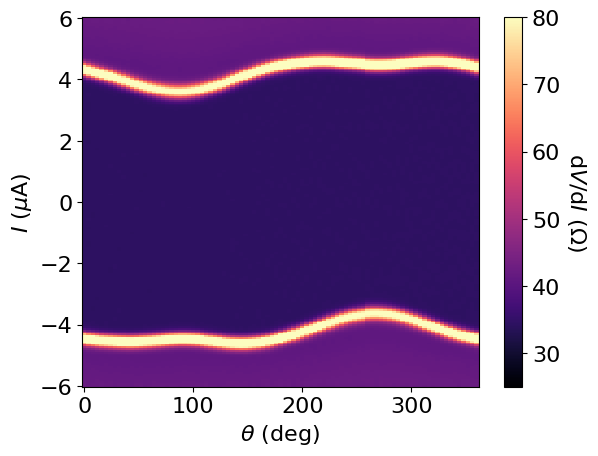
\includegraphics[width=0.32\textwidth]{dVdIthetasweep_55.png}
         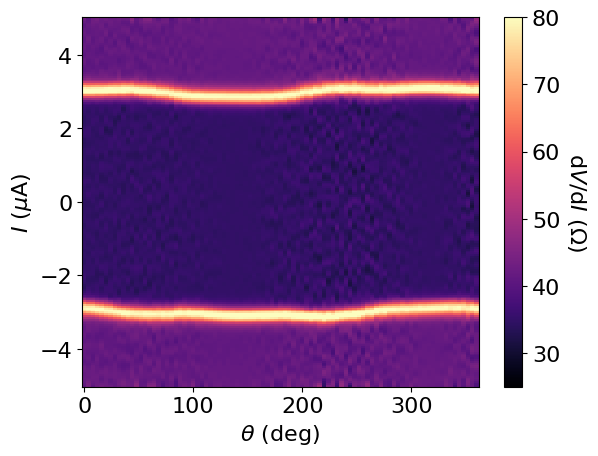
\includegraphics[width=0.32\textwidth]{dVdIthetasweep_71.png}
         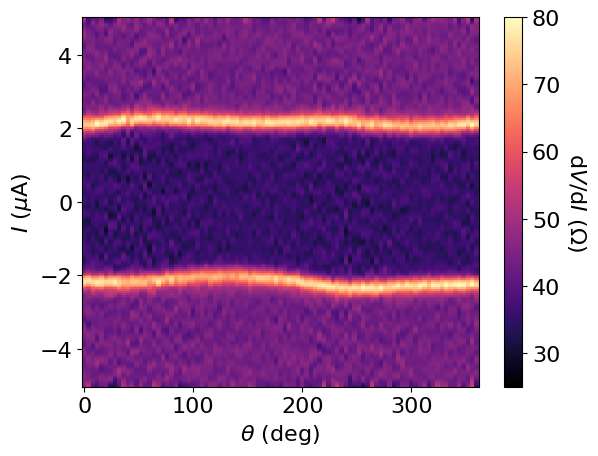
\includegraphics[width=0.32\textwidth]{dVdIthetasweep_72.png}
         %\caption{A portion of the resist is irradiated with an electron beam in as specified pattern.}
         %\label{c}
     \end{subfigure}
        \caption{$\phi$ and $\theta$ sweeps, corresponding to the same device in each case.}
        \label{fig:}
        
\end{figure}


\subsubsection*{D2: AuNb, 50 nm Nb}
\subsubsection*{Z Direction, High Field}


\begin{figure}[H]
     \centering
     \begin{subfigure}[b]{\textwidth}
         \centering
         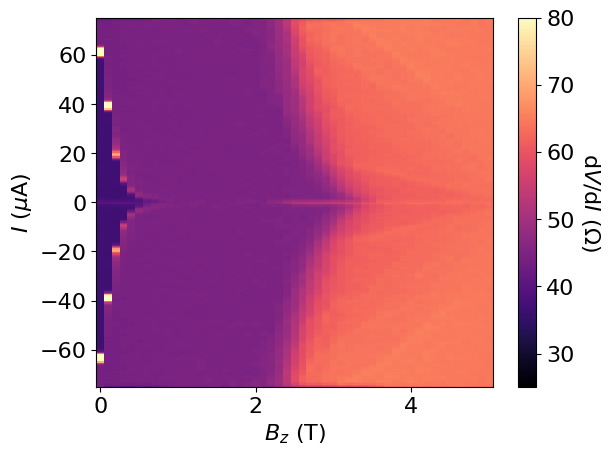
\includegraphics[width=0.32\textwidth]{Appendix_D/D2/dVdIBZ_109.png}
         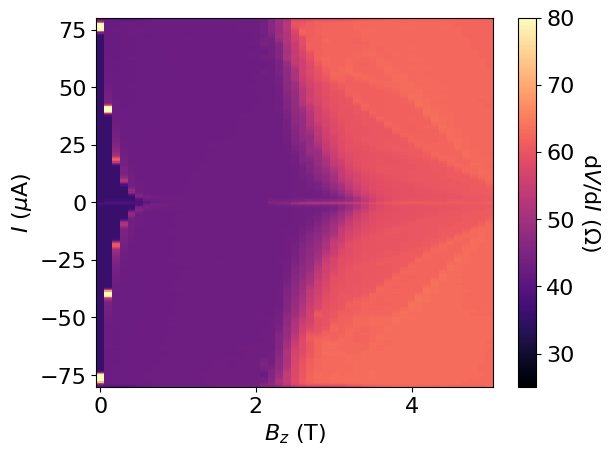
\includegraphics[width=0.32\textwidth]{Appendix_D/D2/dVdIBZ_196.png}
         %\caption{A portion of the resist is irradiated with an electron beam in as specified pattern.}
         %\label{c}
     \end{subfigure}
	 \caption{Out of plane BVI measurements.}
     \label{fig:}
        
\end{figure}

\subsubsection*{X,Y,Z directions, Low field}

\begin{figure}[H]
     \centering
     \begin{subfigure}[b]{\textwidth}
         \centering
         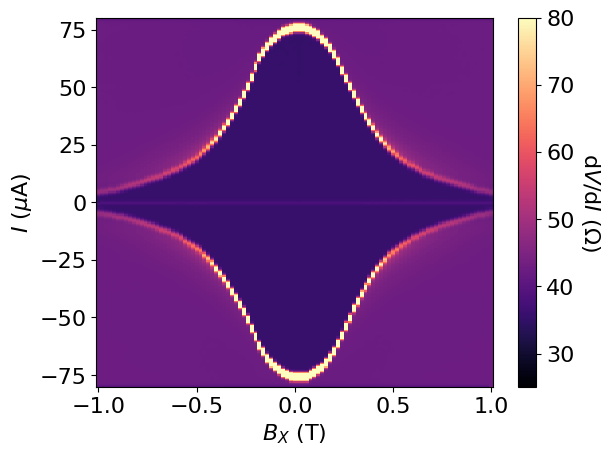
\includegraphics[width=0.32\textwidth]{Appendix_D/D2/dVdIBX_201.png}
         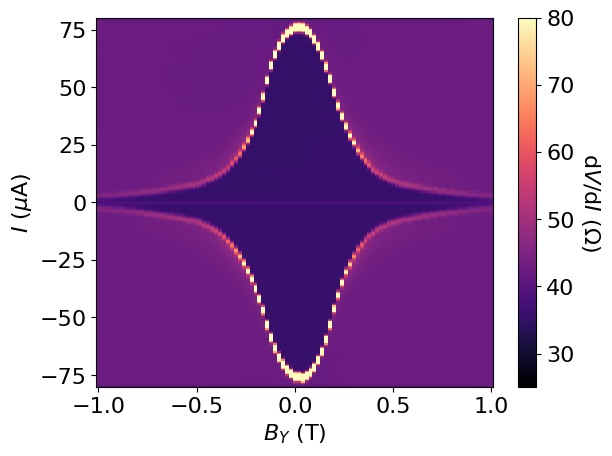
\includegraphics[width=0.32\textwidth]{Appendix_D/D2/dVdIBY_200.png}
         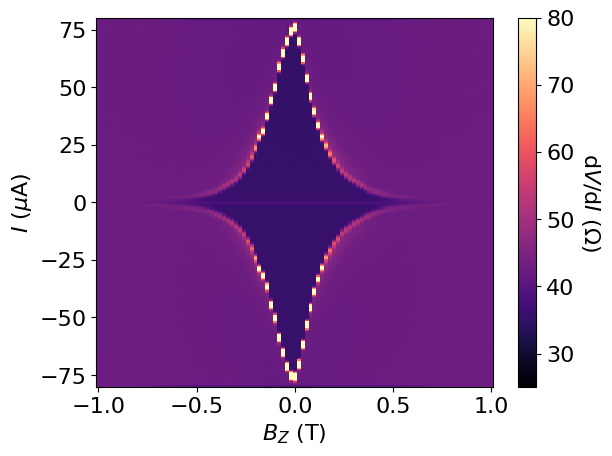
\includegraphics[width=0.32\textwidth]{Appendix_D/D2/dVdIBZ_198.png}
         %\caption{A portion of the resist is irradiated with an electron beam in as specified pattern.}
         %\label{c}
     \end{subfigure}
	 \caption{BVI measurements in the X, Y and Z directions.}
     \label{fig:}
        
\end{figure}

\subsubsection*{$\phi$-Sweep}

\begin{figure}[H]
     \centering
     \begin{subfigure}[b]{\textwidth}
         \centering
         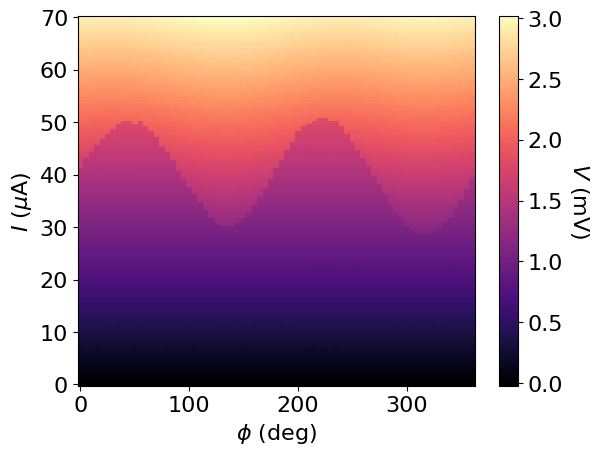
\includegraphics[width=0.32\textwidth]{Appendix_D/D2/phisweep_79.png}
         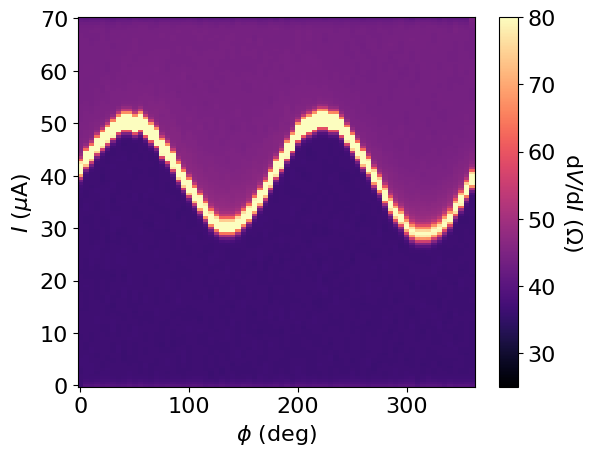
\includegraphics[width=0.32\textwidth]{Appendix_D/D2/dVdIphisweep_79.png}
         %\caption{A portion of the resist is irradiated with an electron beam in as specified pattern.}
         %\label{c}
     \end{subfigure}
     
        \caption{$\phi$ and $\theta$ sweeps, corresponding to the same device.}
        \label{fig:}
        
\end{figure}

\subsubsection*{D3: AuNb, 60 nm Spacing}
\subsubsection*{Z Direction, High Field}



\begin{figure}[H]
     \centering
     \begin{subfigure}[b]{\textwidth}
         \centering
         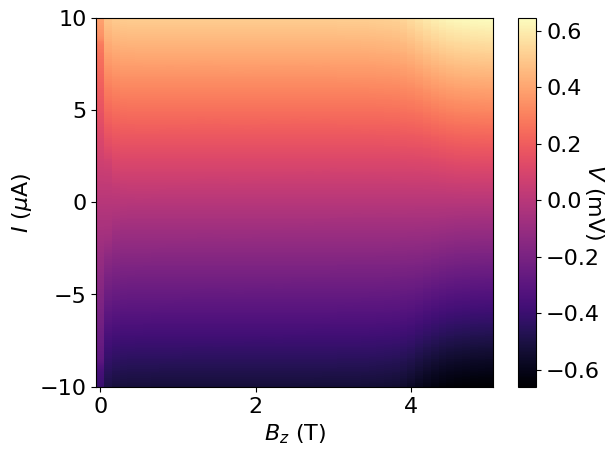
\includegraphics[width=0.32\textwidth]{Appendix_D/D3/VIBZ_17.png}
         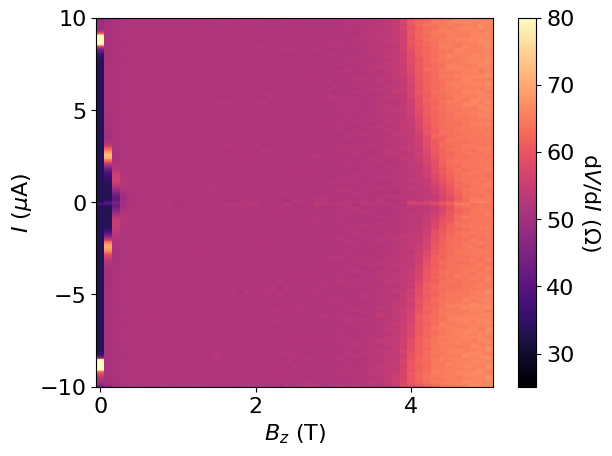
\includegraphics[width=0.32\textwidth]{Appendix_D/D3/dVdIBZ_17.png}
         %\caption{A portion of the resist is irradiated with an electron beam in as specified pattern.}
         %\label{c}
     \end{subfigure}
     
        \caption{Out of plane BVI measurements.}
        \label{fig:}
        
\end{figure}
\subsubsection*{X,Y,Z directions, Low field}

\begin{figure}[H]
     \centering
     \begin{subfigure}[b]{\textwidth}
         \centering
         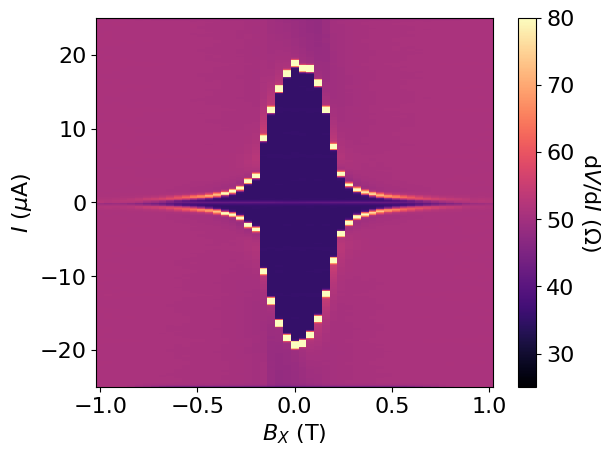
\includegraphics[width=0.32\textwidth]{Appendix_D/D3/dVdIBX_41.png}
         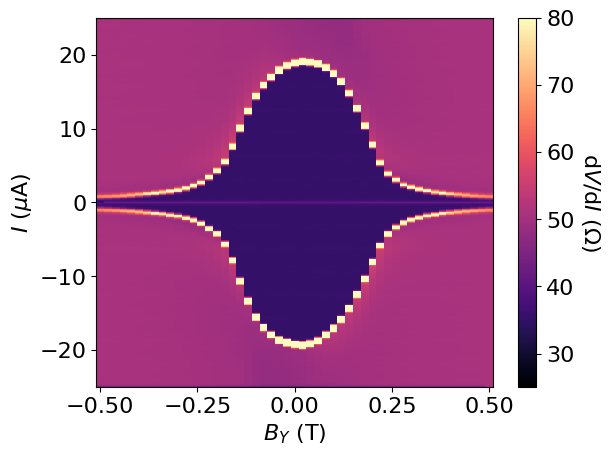
\includegraphics[width=0.32\textwidth]{Appendix_D/D3/dVdIBY_42.png}
         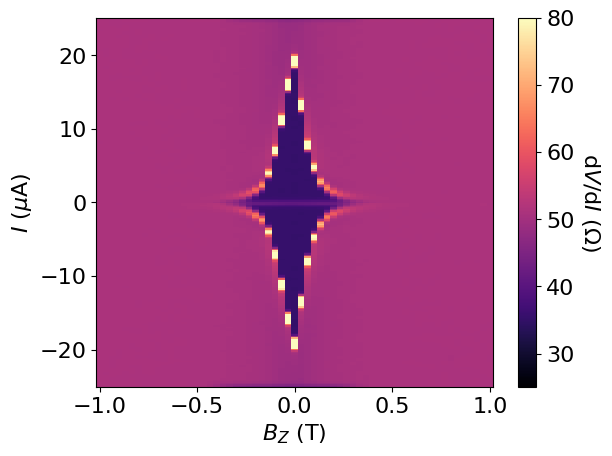
\includegraphics[width=0.32\textwidth]{Appendix_D/D3/dVdIBZ_64.png}
         %\caption{A portion of the resist is irradiated with an electron beam in as specified pattern.}
         %\label{c}
     \end{subfigure}
	 \caption{BVI measurements in the X, Y and Z directions.}
     \label{fig:}
        
\end{figure}

\subsubsection*{$\phi$-Sweep}

\begin{figure}[H]
     \centering
     \begin{subfigure}[b]{\textwidth}
         \centering
         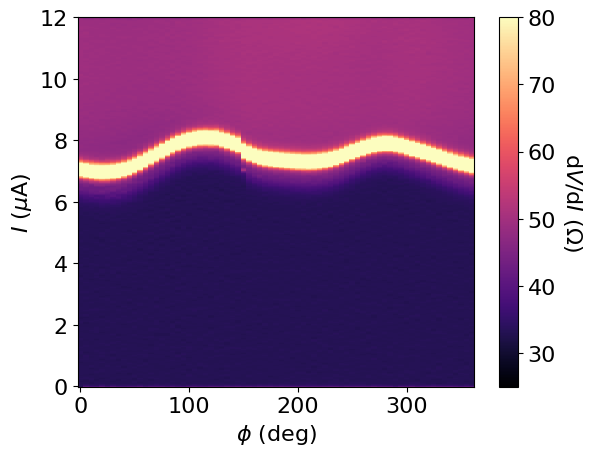
\includegraphics[width=0.32\textwidth]{Appendix_D/D3/dVdIphisweep_22.png}
         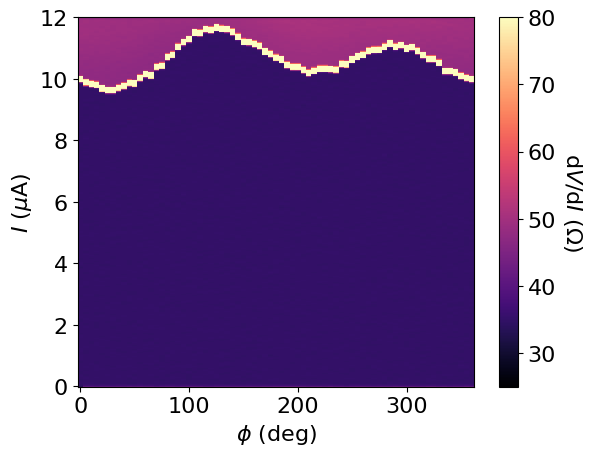
\includegraphics[width=0.32\textwidth]{Appendix_D/D3/dVdIphisweep_23.png}
         %\caption{A portion of the resist is irradiated with an electron beam in as specified pattern.}
         %\label{c}
     \end{subfigure}
	 \caption{$\phi$ and $\theta$ sweeps, corresponding to the same device.}
     \label{fig:}
        
\end{figure}


\subsubsection*{D4: AuNb, 60 nm Spacing}


\subsection{E: Electromigration Curves}
\subsubsection*{E1: PdNb}


\begin{figure}[H]
     \centering
     \begin{subfigure}[b]{\textwidth}
         \centering
         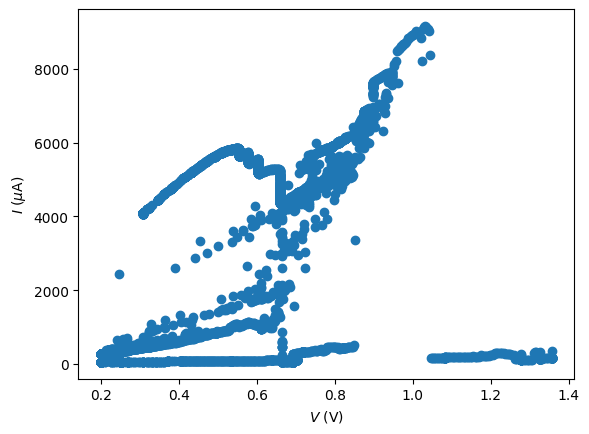
\includegraphics[width=0.32\textwidth]{MigrationIV_A1.png}
         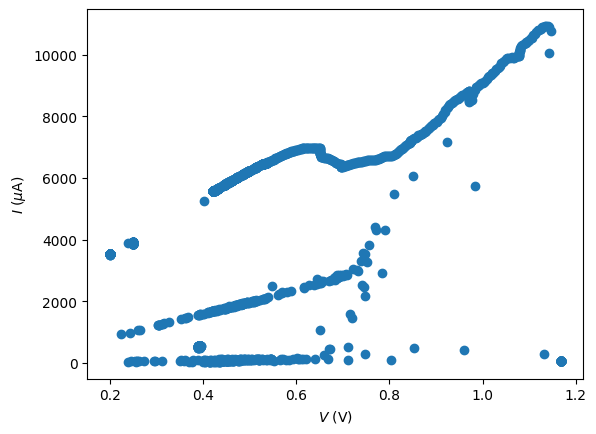
\includegraphics[width=0.32\textwidth]{MigrationIV_B1.png}
         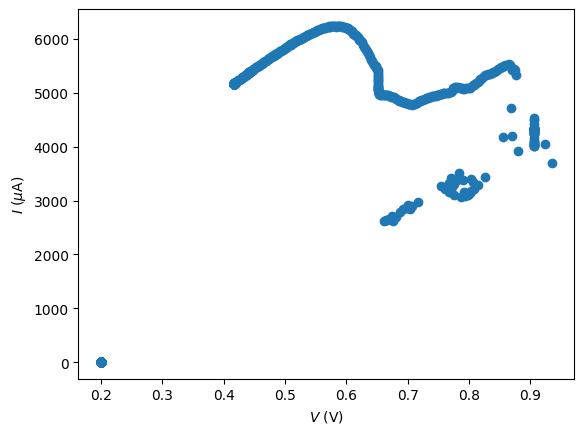
\includegraphics[width=0.32\textwidth]{MigrationIV_B8.png}
         %\caption{A portion of the resist is irradiated with an electron beam in as specified pattern.}
         %\label{c}
     \end{subfigure}
     %\hfill
     \begin{subfigure}[b]{\textwidth}
         \centering
         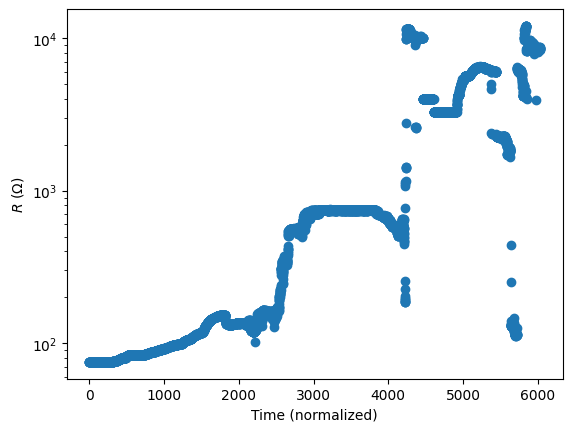
\includegraphics[width=0.32\textwidth]{MigrationRt_A1.png}
         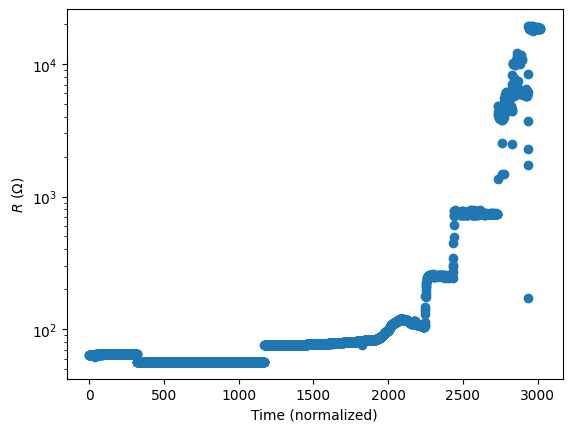
\includegraphics[width=0.32\textwidth]{MigrationRt_B1.png}
         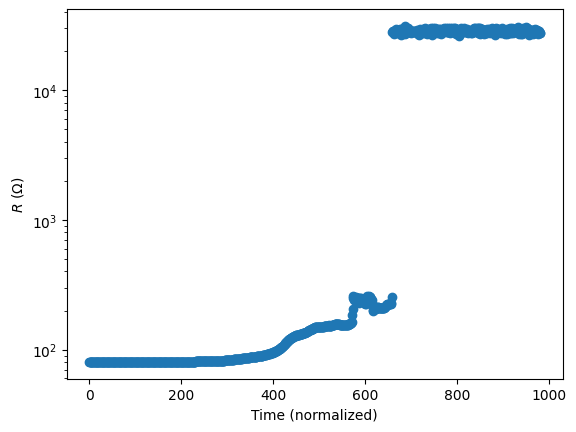
\includegraphics[width=0.32\textwidth]{MigrationRt_B8.png}
         %\caption{A portion of the resist is irradiated with an electron beam in as specified pattern.}
         %\label{c}
     \end{subfigure}
        \caption{Representative electromigration curves.}
        \label{fig:}
        
\end{figure}

\subsubsection*{E2: AuNb, 100 nm Nb}

\begin{figure}[H]
     \centering
     \begin{subfigure}[b]{\textwidth}
         \centering
         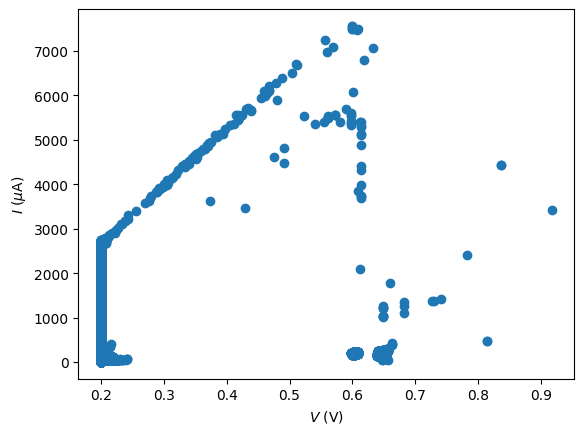
\includegraphics[width=0.32\textwidth]{Appendix_E/E2/MigrationIV_A1.png}
         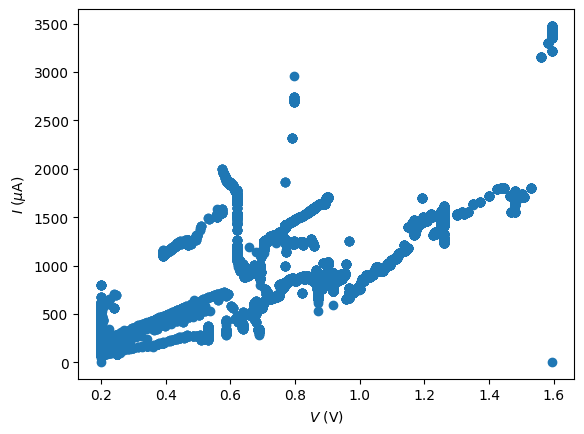
\includegraphics[width=0.32\textwidth]{Appendix_E/E2/MigrationIV_D8.png}
         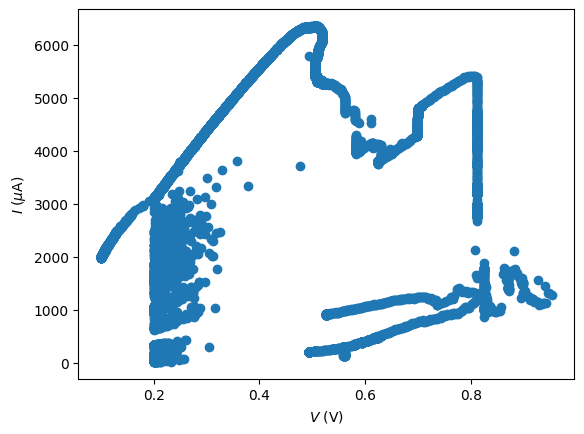
\includegraphics[width=0.32\textwidth]{Appendix_E/E2/MigrationIV_E8.png}
         %\caption{A portion of the resist is irradiated with an electron beam in as specified pattern.}
         %\label{c}
     \end{subfigure}
     %\hfill
     \begin{subfigure}[b]{\textwidth}
         \centering
         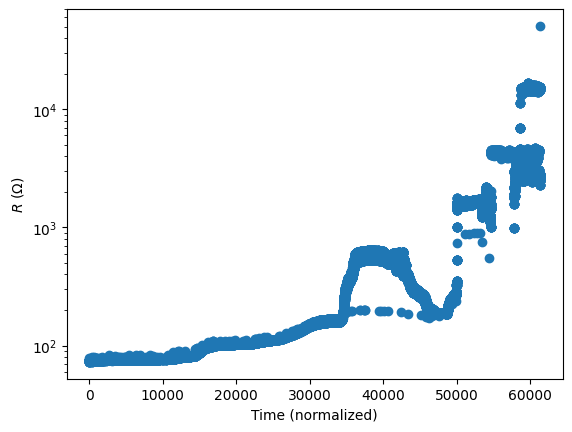
\includegraphics[width=0.32\textwidth]{Appendix_E/E2/MigrationRt_A1.png}
         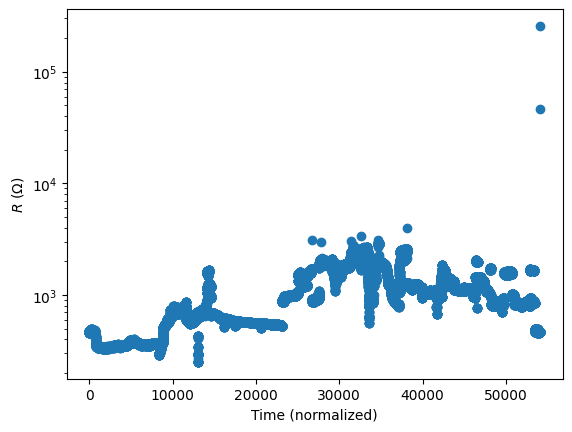
\includegraphics[width=0.32\textwidth]{Appendix_E/E2/MigrationRt_D8.png}
         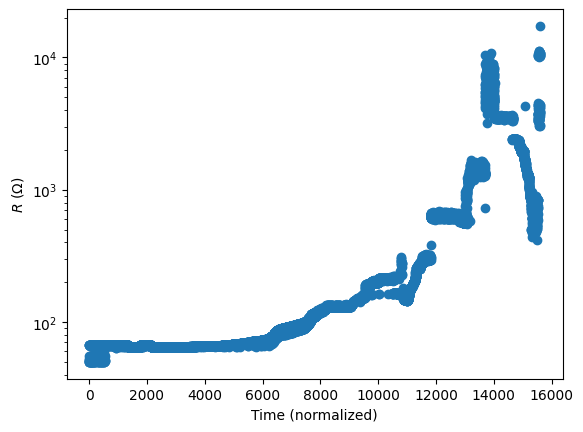
\includegraphics[width=0.32\textwidth]{Appendix_E/E2/MigrationRt_E8.png}
         %\caption{A portion of the resist is irradiated with an electron beam in as specified pattern.}
         %\label{c}
     \end{subfigure}
        \caption{Representative electromigration curves.}
        \label{fig:}
        
\end{figure}

\subsubsection*{E3: AuNb, 50 nm Nb}


\begin{figure}[H]
     \centering
     \begin{subfigure}[b]{\textwidth}
         \centering
         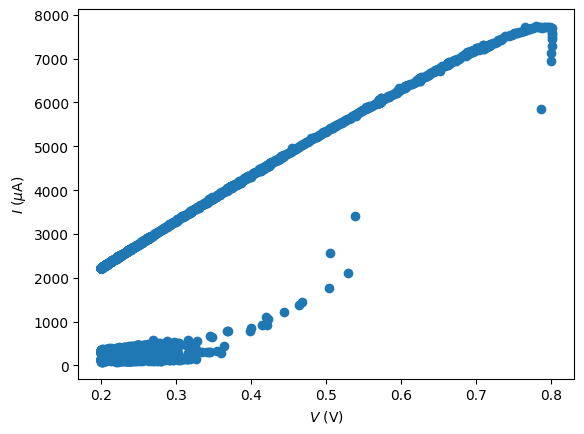
\includegraphics[width=0.32\textwidth]{Appendix_E/E3/MigrationIV_1.png}
         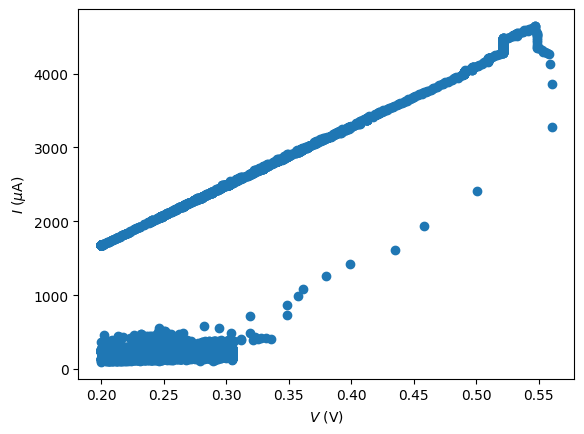
\includegraphics[width=0.32\textwidth]{Appendix_E/E3/MigrationIV_2.png}
         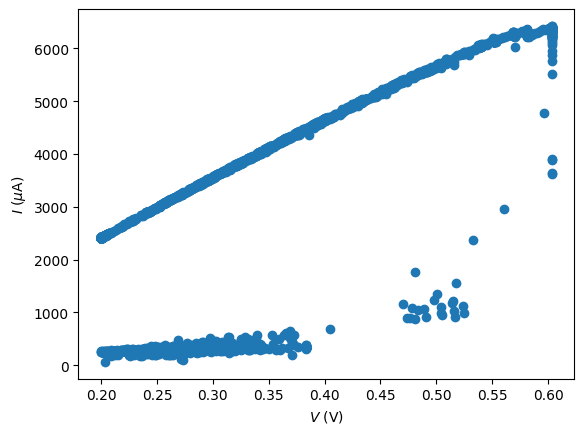
\includegraphics[width=0.32\textwidth]{Appendix_E/E3/MigrationIV_3.png}
         %\caption{A portion of the resist is irradiated with an electron beam in as specified pattern.}
         %\label{c}
     \end{subfigure}
     %\hfill
     \begin{subfigure}[b]{\textwidth}
         \centering
         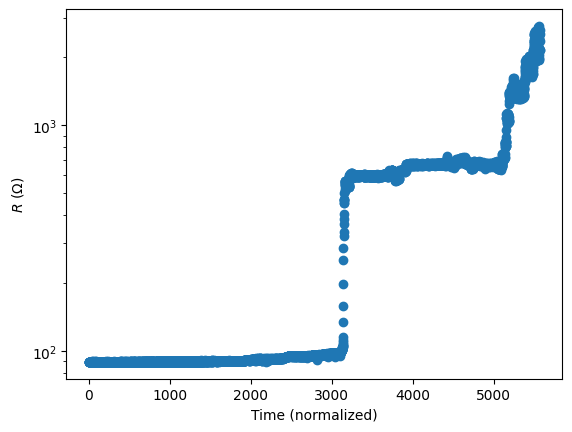
\includegraphics[width=0.32\textwidth]{Appendix_E/E3/MigrationRt_1.png}
         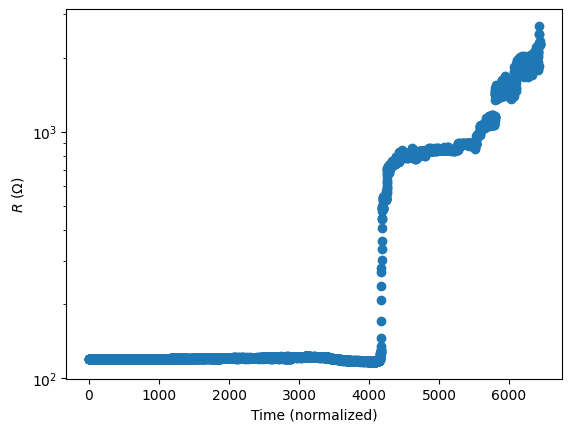
\includegraphics[width=0.32\textwidth]{Appendix_E/E3/MigrationRt_2.png}
         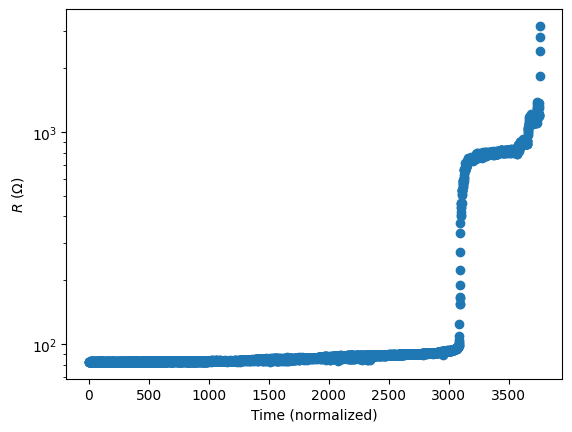
\includegraphics[width=0.32\textwidth]{Appendix_E/E3/MigrationRt_3.png}
         %\caption{A portion of the resist is irradiated with an electron beam in as specified pattern.}
         %\label{c}
     \end{subfigure}
        \caption{Representative electromigration curves.}
        \label{fig:}
        
\end{figure}

\subsubsection*{E4: AuNb, 60 nm Spacing}


\begin{figure}[H]
     \centering
     \begin{subfigure}[b]{\textwidth}
         \centering
         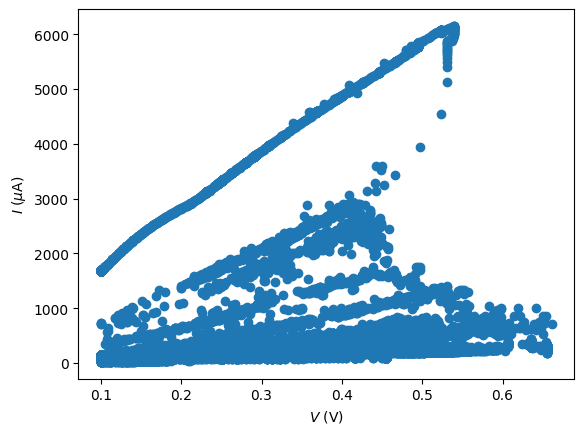
\includegraphics[width=0.32\textwidth]{Appendix_E/E4/MigrationIV_B1.png}
         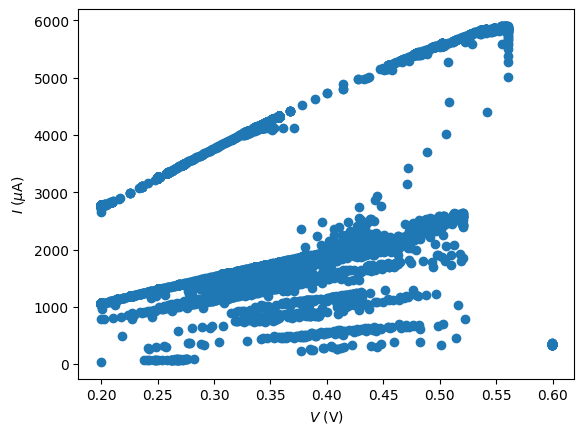
\includegraphics[width=0.32\textwidth]{Appendix_E/E4/MigrationIV_C4.png}
         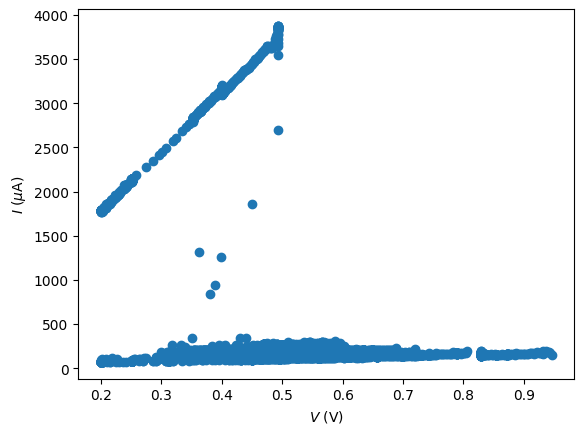
\includegraphics[width=0.32\textwidth]{Appendix_E/E4/MigrationIV_D3.png}
         %\caption{A portion of the resist is irradiated with an electron beam in as specified pattern.}
         %\label{c}
     \end{subfigure}
     %\hfill
     \begin{subfigure}[b]{\textwidth}
         \centering
         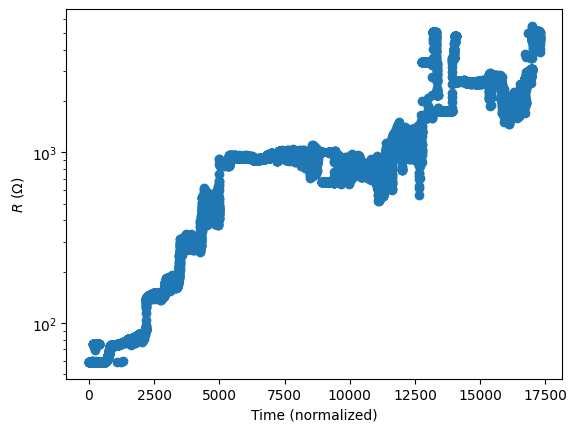
\includegraphics[width=0.32\textwidth]{Appendix_E/E4/MigrationRt_B1.png}
         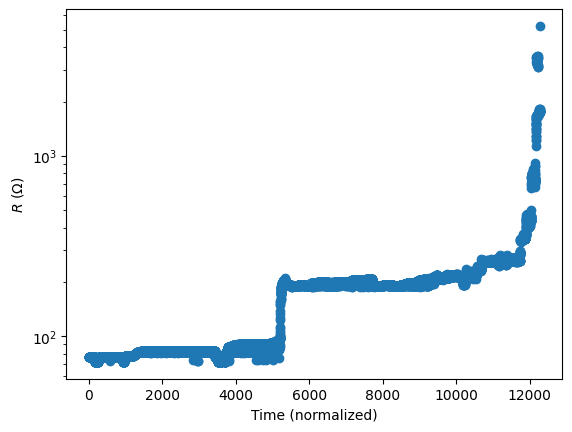
\includegraphics[width=0.32\textwidth]{Appendix_E/E4/MigrationRt_C4.png}
         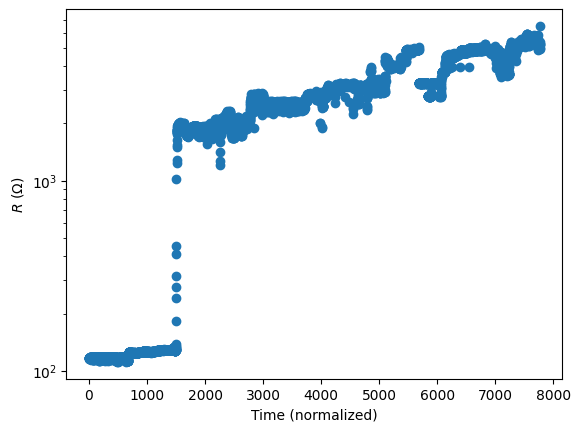
\includegraphics[width=0.32\textwidth]{Appendix_E/E4/MigrationRt_D3.png}
         %\caption{A portion of the resist is irradiated with an electron beam in as specified pattern.}
         %\label{c}
     \end{subfigure}
        \caption{Representative electromigration curves. Since these devices were migrated in stages, the graphs look more chaotic.}
        \label{fig:}
        
\end{figure}

